    %********************************************%
%*       Generated from PreTeXt source      *%
%*       on 2025-01-16T15:12:28-05:00       *%
%*   A recent stable commit (2022-07-01):   *%
%* 6c761d3dba23af92cba35001c852aac04ae99a5f *%
%*                                          *%
%*         https://pretextbook.org          *%
%*                                          *%
%********************************************%
\documentclass[twoside,20pt]{extarticle}
%% Custom Preamble Entries, early (use latex.preamble.early)
%% Always open on odd page
%%   The following adjusts cleardoublepage to remove twosided
%%   check so that we open on odd pages even in one-sided mode
%%   by adding an extra blank page on the preceding even page.
\makeatletter%
\def\cleardoublepage{%
\clearpage\ifodd\c@page\else\thispagestyle{empty}\hbox{}\newpage\if@twocolumn\hbox{}\newpage\fi\fi%
}
\makeatother%
%% Default LaTeX packages
%%   1.  always employed (or nearly so) for some purpose, or
%%   2.  a stylewriter may assume their presence
\usepackage{geometry}
%% Some aspects of the preamble are conditional,
%% the LaTeX engine is one such determinant
\usepackage{ifthen}
%% etoolbox has a variety of modern conveniences
\usepackage{etoolbox}
\usepackage{ifxetex,ifluatex}
%% Raster graphics inclusion
\usepackage{graphicx}
%% Color support, xcolor package
%% Always loaded, for: add/delete text, author tools
%% Here, since tcolorbox loads tikz, and tikz loads xcolor
\PassOptionsToPackage{dvipsnames,svgnames,table}{xcolor}
\usepackage{xcolor}
%% begin: defined colors, via xcolor package, for styling
%% end: defined colors, via xcolor package, for styling
%% Colored boxes, and much more, though mostly styling
%% skins library provides "enhanced" skin, employing tikzpicture
%% boxes may be configured as "breakable" or "unbreakable"
%% "raster" controls grids of boxes, aka side-by-side
\usepackage{tcolorbox}
\tcbuselibrary{skins}
\tcbuselibrary{breakable}
\tcbuselibrary{raster}
%% We load some "stock" tcolorbox styles that we use a lot
%% Placement here is provisional, there will be some color work also
%% First, black on white, no border, transparent, but no assumption about titles
\tcbset{ bwminimalstyle/.style={size=minimal, boxrule=0pt, frame empty,
colback=white, colbacktitle=white, coltitle=black, opacityfill=0.0} }
%% Second, bold title, run-in to text/paragraph/heading
%% Space afterwards will be controlled by environment,
%% independent of constructions of the tcb title
%% Places \blocktitlefont onto many block titles
\tcbset{ runintitlestyle/.style={fonttitle=\blocktitlefont\upshape\bfseries, attach title to upper} }
%% Spacing prior to each exercise, anywhere
\tcbset{ exercisespacingstyle/.style={before skip={1.5ex plus 0.5ex}} }
%% Spacing prior to each block
\tcbset{ blockspacingstyle/.style={before skip={0ex plus 0ex minus 0ex}, before upper={\setlength{\parskip}{1.5ex}\renewcommand{\\}{\par\vspace*{-0.8\parskip}}}}}
%% xparse allows the construction of more robust commands,
%% this is a necessity for isolating styling and behavior
%% The tcolorbox library of the same name loads the base library
\tcbuselibrary{xparse}
%% The tcolorbox library loads TikZ, its calc package is generally useful,
%% and is necessary for some smaller documents that use partial tcolor boxes
%% See:  https://github.com/PreTeXtBook/pretext/issues/1624
\usetikzlibrary{calc}
%% We use some more exotic tcolorbox keys to restore indentation to parboxes
\tcbuselibrary{hooks}
%% Save default paragraph indentation and parskip for use later, when adjusting parboxes
\newlength{\normalparindent}
\newlength{\normalparskip}
\AtBeginDocument{\setlength{\normalparindent}{\parindent}}
\AtBeginDocument{\setlength{\normalparskip}{\parskip}}
\newcommand{\setparstyle}{\setlength{\parindent}{\normalparindent}\setlength{\parskip}{\normalparskip}}%% Hyperref should be here, but likes to be loaded late
%%
%% Inline math delimiters, \(, \), need to be robust
%% 2016-01-31:  latexrelease.sty  supersedes  fixltx2e.sty
%% If  latexrelease.sty  exists, bugfix is in kernel
%% If not, bugfix is in  fixltx2e.sty
%% See:  https://tug.org/TUGboat/tb36-3/tb114ltnews22.pdf
%% and read "Fewer fragile commands" in distribution's  latexchanges.pdf
\IfFileExists{latexrelease.sty}{}{\usepackage{fixltx2e}}
%% shorter subnumbers in some side-by-side require manipulations
\usepackage{xstring}
%% Footnote counters and part/chapter counters are manipulated
%% April 2018:  chngcntr  commands now integrated into the kernel,
%% but circa 2018/2019 the package would still try to redefine them,
%% so we need to do the work of loading conditionally for old kernels.
%% From version 1.1a,  chngcntr  should detect defintions made by LaTeX kernel.
\ifdefined\counterwithin
\else
    \usepackage{chngcntr}
\fi
%% Text height identically 9 inches, text width varies on point size
%% See Bringhurst 2.1.1 on measure for recommendations
%% 75 characters per line (count spaces, punctuation) is target
%% which is the upper limit of Bringhurst's recommendations
\geometry{letterpaper, inner=1.2in, outer=0.7in, top=0.35in, bottom=0.7in}
%% Custom Page Layout Adjustments (use publisher page-geometry entry)
%% This LaTeX file may be compiled with pdflatex, xelatex, or lualatex executables
%% LuaTeX is not explicitly supported, but we do accept additions from knowledgeable users
%% The conditional below provides  pdflatex  specific configuration last
%% begin: engine-specific capabilities
\ifthenelse{\boolean{xetex} \or \boolean{luatex}}{%
%% begin: xelatex and lualatex-specific default configuration
\ifxetex\usepackage{xltxtra}\fi
%% realscripts is the only part of xltxtra relevant to lualatex 
\ifluatex\usepackage{realscripts}\fi
%% end:   xelatex and lualatex-specific default configuration
}{
%% begin: pdflatex-specific default configuration
%% We assume a PreTeXt XML source file may have Unicode characters
%% and so we ask LaTeX to parse a UTF-8 encoded file
%% This may work well for accented characters in Western language,
%% but not with Greek, Asian languages, etc.
%% When this is not good enough, switch to the  xelatex  engine
%% where Unicode is better supported (encouraged, even)
\usepackage[utf8]{inputenc}
%% end: pdflatex-specific default configuration
}
%% end:   engine-specific capabilities
%%
%% Fonts.  Conditional on LaTex engine employed.
%% Default Text Font: The Latin Modern fonts are
%% "enhanced versions of the [original TeX] Computer Modern fonts."
%% We use them as the default text font for PreTeXt output.
%% Automatic Font Control
%% Portions of a document, are, or may, be affected by defined commands
%% These are perhaps more flexible when using  xelatex  rather than  pdflatex
%% The following definitions are meant to be re-defined in a style, using \renewcommand
%% They are scoped when employed (in a TeX group), and so should not be defined with an argument
\newcommand{\divisionfont}{\relax}
\newcommand{\blocktitlefont}{\relax}
\newcommand{\contentsfont}{\relax}
\newcommand{\pagefont}{\relax}
\newcommand{\tabularfont}{\relax}
\newcommand{\xreffont}{\relax}
\newcommand{\titlepagefont}{\relax}
%%
\ifthenelse{\boolean{xetex} \or \boolean{luatex}}{%
%% begin: font setup and configuration for use with xelatex
%% Generally, xelatex is necessary for non-Western fonts
%% fontspec package provides extensive control of system fonts,
%% meaning *.otf (OpenType), and apparently *.ttf (TrueType)
%% that live *outside* your TeX/MF tree, and are controlled by your *system*
%% (it is possible that a TeX distribution will place fonts in a system location)
%%
%% The fontspec package is the best vehicle for using different fonts in  xelatex
%% So we load it always, no matter what a publisher or style might want
%%
\usepackage{fontspec}
%%
%% begin: xelatex main font ("font-xelatex-main" template)
%% Latin Modern Roman is the default font for xelatex and so is loaded with a TU encoding
%% *in the format* so we can't touch it, only perhaps adjust it later
%% in one of two ways (then known by NFSS names such as "lmr")
%% (1) via NFSS with font family names such as "lmr" and "lmss"
%% (2) via fontspec with commands like \setmainfont{Latin Modern Roman}
%% The latter requires the font to be known at the system-level by its font name,
%% but will give access to OTF font features through optional arguments
%% https://tex.stackexchange.com/questions/470008/
%% where-and-how-does-fontspec-sty-specify-the-default-font-latin-modern-roman
%% http://tex.stackexchange.com/questions/115321
%% /how-to-optimize-latin-modern-font-with-xelatex
%%
%% end:   xelatex main font ("font-xelatex-main" template)
%% begin: xelatex mono font ("font-xelatex-mono" template)
%% (conditional on non-trivial uses being present in source)
%% end:   xelatex mono font ("font-xelatex-mono" template)
%% begin: xelatex font adjustments ("font-xelatex-style" template)
%% end:   xelatex font adjustments ("font-xelatex-style" template)
%%
%% Extensive support for other languages
\usepackage{polyglossia}
%% Set main/default language based on pretext/@xml:lang value
%% document language code is "es-ES", Spanish
\setmainlanguage{spanish}
%% Enable secondary languages based on discovery of @xml:lang values
%% Enable fonts/scripts based on discovery of @xml:lang values
%% Western languages should be ably covered by Latin Modern Roman
%% end:   font setup and configuration for use with xelatex
}{%
%% begin: font setup and configuration for use with pdflatex
%% begin: pdflatex main font ("font-pdflatex-main" template)
\usepackage{lmodern}
\usepackage[T1]{fontenc}
%% end:   pdflatex main font ("font-pdflatex-main" template)
%% begin: pdflatex mono font ("font-pdflatex-mono" template)
%% (conditional on non-trivial uses being present in source)
%% end:   pdflatex mono font ("font-pdflatex-mono" template)
%% begin: pdflatex font adjustments ("font-pdflatex-style" template)
%% end:   pdflatex font adjustments ("font-pdflatex-style" template)
%% end:   font setup and configuration for use with pdflatex
}
%% Micromanage spacing, etc.  The named "microtype-options"
%% template may be employed to fine-tune package behavior
\usepackage{microtype}
%% Symbols, align environment, commutative diagrams, bracket-matrix
\usepackage{amsmath}
\usepackage{amscd}
\usepackage{amssymb}
%% allow page breaks within display mathematics anywhere
%% level 4 is maximally permissive
%% this is exactly the opposite of AMSmath package philosophy
%% there are per-display, and per-equation options to control this
%% split, aligned, gathered, and alignedat are not affected
\allowdisplaybreaks[4]
%% allow more columns to a matrix
%% can make this even bigger by overriding with  latex.preamble.late  processing option
\setcounter{MaxMatrixCols}{30}
%%
%%
%% Division Titles, and Page Headers/Footers
%% titlesec package, loading "titleps" package cooperatively
%% See code comments about the necessity and purpose of "explicit" option.
%% The "newparttoc" option causes a consistent entry for parts in the ToC 
%% file, but it is only effective if there is a \titleformat for \part.
%% "pagestyles" loads the  titleps  package cooperatively.
\usepackage[explicit, newparttoc, pagestyles]{titlesec}
%% The companion titletoc package for the ToC.
\usepackage{titletoc}
%% begin: customizations of page styles via the modal "titleps-style" template
%% Designed to use commands from the LaTeX "titleps" package
\pagestyle{plain}
%% end: customizations of page styles via the modal "titleps-style" template
%%
%% Create globally-available macros to be provided for style writers
%% These are redefined for each occurence of each division
\newcommand{\divisionnameptx}{\relax}%
\newcommand{\titleptx}{\relax}%
\newcommand{\subtitleptx}{\relax}%
\newcommand{\shortitleptx}{\relax}%
\newcommand{\authorsptx}{\relax}%
\newcommand{\epigraphptx}{\relax}%
%% Create environments for possible occurences of each division
%% Environment for a PTX "section" at the level of a LaTeX "section"
\NewDocumentEnvironment{sectionptx}{mmmmmmm}
{%
\renewcommand{\divisionnameptx}{#1}%
\renewcommand{\titleptx}{#2}%
\renewcommand{\subtitleptx}{#3}%
\renewcommand{\shortitleptx}{#4}%
\renewcommand{\authorsptx}{#5}%
\renewcommand{\epigraphptx}{#6}%
\clearpage
\vspace*{8cm}
\section[{#4}]{#2}%
\vfill
\label{#7}%
}{}%
%% Environment for a PTX "subsection" at the level of a LaTeX "subsection"
\NewDocumentEnvironment{subsectionptx}{mmmmmmm}
{%
\renewcommand{\divisionnameptx}{#1}%
\renewcommand{\titleptx}{#2}%
\renewcommand{\subtitleptx}{#3}%
\renewcommand{\shortitleptx}{#4}%
\renewcommand{\authorsptx}{#5}%
\renewcommand{\epigraphptx}{#6}%
\newpage
\subsection[{#4}]{#2}%
\vspace{-0.3cm}%
\label{#7}%
}{}%
%% Environment for a PTX "subsubsection" at the level of a LaTeX "subsubsection"
\NewDocumentEnvironment{subsubsectionptx}{mmmmmmm}
{%
\renewcommand{\divisionnameptx}{#1}%
\renewcommand{\titleptx}{#2}%
\renewcommand{\subtitleptx}{#3}%
\renewcommand{\shortitleptx}{#4}%
\renewcommand{\authorsptx}{#5}%
\renewcommand{\epigraphptx}{#6}%
% \vspace{-0.4cm}
\subsubsection[{#4}]{#2}\nobreak%
% \vspace{-0.4cm}
\label{#7}%
}{}%
%% Environment for a PTX "exercises" at the level of a LaTeX "subsection"
\NewDocumentEnvironment{exercises-subsection}{mmmmmmm}
{%
\renewcommand{\divisionnameptx}{#1}%
\renewcommand{\titleptx}{#2}%
\renewcommand{\subtitleptx}{#3}%
\renewcommand{\shortitleptx}{#4}%
\renewcommand{\authorsptx}{#5}%
\renewcommand{\epigraphptx}{#6}%
\clearpage
\subsection[{#4}]{#2}%
\label{#7}%
}{}%
%% Environment for a PTX "exercises" at the level of a LaTeX "subsection"
\NewDocumentEnvironment{exercises-subsection-numberless}{mmmmmmm}
{%
\renewcommand{\divisionnameptx}{#1}%
\renewcommand{\titleptx}{#2}%
\renewcommand{\subtitleptx}{#3}%
\renewcommand{\shortitleptx}{#4}%
\renewcommand{\authorsptx}{#5}%
\renewcommand{\epigraphptx}{#6}%
\subsection*{#2}%
\addcontentsline{toc}{subsection}{#4}
\label{#7}%
}{}%
%% Environment for a PTX "references" at the level of a LaTeX "subsection"
\NewDocumentEnvironment{references-subsection}{mmmmmmm}
{%
\renewcommand{\divisionnameptx}{#1}%
\renewcommand{\titleptx}{#2}%
\renewcommand{\subtitleptx}{#3}%
\renewcommand{\shortitleptx}{#4}%
\renewcommand{\authorsptx}{#5}%
\renewcommand{\epigraphptx}{#6}%
\newpage
\subsection[{#4}]{#2}%
\label{#7}%
}{}%
%% Environment for a PTX "references" at the level of a LaTeX "subsection"
\NewDocumentEnvironment{references-subsection-numberless}{mmmmmmm}
{%
\renewcommand{\divisionnameptx}{#1}%
\renewcommand{\titleptx}{#2}%
\renewcommand{\subtitleptx}{#3}%
\renewcommand{\shortitleptx}{#4}%
\renewcommand{\authorsptx}{#5}%
\renewcommand{\epigraphptx}{#6}%
\newpage
\subsection*{#2}%
\addcontentsline{toc}{subsection}{#4}
\label{#7}%
}{}%
%% Environment for a PTX "reading-questions" at the level of a LaTeX "subsubsection"
\NewDocumentEnvironment{reading-questions-subsubsection}{mmmmmmm}
{%
\renewcommand{\divisionnameptx}{#1}%
\renewcommand{\titleptx}{#2}%
\renewcommand{\subtitleptx}{#3}%
\renewcommand{\shortitleptx}{#4}%
\renewcommand{\authorsptx}{#5}%
\renewcommand{\epigraphptx}{#6}%
% \vspace{-0.4cm}
% \subsubsection[{#4}]{#2}\nobreak%
% \vspace{-0.4cm}
\label{#7}%
}{}%
%% Environment for a PTX "reading-questions" at the level of a LaTeX "subsubsection"
\NewDocumentEnvironment{reading-questions-subsubsection-numberless}{mmmmmmm}
{%
\renewcommand{\divisionnameptx}{#1}%
\renewcommand{\titleptx}{#2}%
\renewcommand{\subtitleptx}{#3}%
\renewcommand{\shortitleptx}{#4}%
\renewcommand{\authorsptx}{#5}%
\renewcommand{\epigraphptx}{#6}%
\subsubsection*{#2}\nobreak%
\addcontentsline{toc}{subsubsection}{#4}
\label{#7}%
}{}%
%% Environment for a PTX "references" at the level of a LaTeX "section"
\NewDocumentEnvironment{references-section}{mmmmmmm}
{%
\renewcommand{\divisionnameptx}{#1}%
\renewcommand{\titleptx}{#2}%
\renewcommand{\subtitleptx}{#3}%
\renewcommand{\shortitleptx}{#4}%
\renewcommand{\authorsptx}{#5}%
\renewcommand{\epigraphptx}{#6}%
\clearpage
\section[{#4}]{#2}%
\label{#7}%
}{}%
%% Environment for a PTX "references" at the level of a LaTeX "section"
\NewDocumentEnvironment{references-section-numberless}{mmmmmmm}
{%
\renewcommand{\divisionnameptx}{#1}%
\renewcommand{\titleptx}{#2}%
\renewcommand{\subtitleptx}{#3}%
\renewcommand{\shortitleptx}{#4}%
\renewcommand{\authorsptx}{#5}%
\renewcommand{\epigraphptx}{#6}%
\section*{#2}%
\addcontentsline{toc}{section}{#4}
\label{#7}%
}{}%
%%
%% Styles for six traditional LaTeX divisions
\titleformat{\part}[display]
{\divisionfont\Huge\bfseries\centering}{\divisionnameptx\space\thepart}{30pt}{\Huge#1}
[{\Large\centering\authorsptx}]
\titleformat{\chapter}[display]
{\divisionfont\huge\bfseries}{\divisionnameptx\space\thechapter}{20pt}{\Huge#1}
[{\Large\authorsptx}]
\titleformat{name=\chapter,numberless}[display]
{\divisionfont\huge\bfseries}{}{0pt}{#1}
[{\Large\authorsptx}]
\titlespacing*{\chapter}{0pt}{50pt}{40pt}
\titleformat{\section}[hang]
{\raggedright\divisionfont\LARGE\bfseries}{\thesection}{1ex}{#1}
[{\large\authorsptx}]
\titleformat{name=\section,numberless}[block]
{\raggedright\divisionfont\Huge\bfseries}{}{0pt}{#1}
[{\large\authorsptx}]
\titlespacing*{\section}{0pt}{3.5ex plus 1ex minus .2ex}{2.3ex plus .2ex}
\titleformat{\subsection}[hang]
{\raggedright\divisionfont\Large\bfseries}{\thesubsection}{}{#1}
[{\normalsize\authorsptx}]
\titleformat{name=\subsection,numberless}[block]
{\raggedright\divisionfont\Large\bfseries}{}{0pt}{#1}
[{\normalsize\authorsptx}]
\titlespacing*{\subsection}{0pt}{0pt}{0.8ex plus 0.2ex minus 0.3ex}
\titleformat{\subsubsection}[hang]
{\divisionfont\normalsize\bfseries}{\thesubsubsection}{1em}{#1}
[{\small\authorsptx}]
\titleformat{name=\subsubsection,numberless}[block]
{\divisionfont\normalsize\bfseries}{}{0pt}{#1}
[{\normalsize\authorsptx}]
\titlespacing*{\subsubsection}{0pt}{0ex minus 0.3ex}{-1ex minus 0.3ex}
\titleformat{\paragraph}[hang]
{\divisionfont\normalsize\bfseries}{\theparagraph}{1em}{#1}
[{\small\authorsptx}]
\titleformat{name=\paragraph,numberless}[block]
{\divisionfont\normalsize\bfseries}{}{0pt}{#1}
[{\normalsize\authorsptx}]
\titlespacing*{\paragraph}{0pt}{3.25ex plus 1ex minus .2ex}{1.5em}
%%
%% Styles for five traditional LaTeX divisions
\titlecontents{part}%
[0pt]{\contentsmargin{0em}\addvspace{1pc}\contentsfont\bfseries}%
{\Large\thecontentslabel\enspace}{\Large}%
{}%
[\addvspace{.5pc}]%
\titlecontents{chapter}%
[0pt]{\contentsmargin{0em}\addvspace{1pc}\contentsfont\bfseries}%
{\large\thecontentslabel\enspace}{\large}%
{\hfill\bfseries\thecontentspage}%
[\addvspace{.5pc}]%
\dottedcontents{section}[3.8em]{\contentsfont}{2.3em}{1pc}%
\dottedcontents{subsection}[6.1em]{\contentsfont}{3.2em}{1pc}%
\dottedcontents{subsubsection}[9.3em]{\contentsfont}{4.3em}{1pc}%
%%
%% Begin: Semantic Macros
%% To preserve meaning in a LaTeX file
%%
%% \mono macro for content of "c", "cd", "tag", etc elements
%% Also used automatically in other constructions
%% Simply an alias for \texttt
%% Always defined, even if there is no need, or if a specific tt font is not loaded
\newcommand{\mono}[1]{\texttt{#1}}
%%
%% Following semantic macros are only defined here if their
%% use is required only in this specific document
%%
%% Used for warnings, typically bold and italic
\newcommand{\alert}[1]{\textbf{\textit{#1}}}
%% Used for fillin answer blank in text
%% Relies on calc package, loaded via tcolorbox
%% Argument is intended number of characters of blank
%% Length may compress for output to fit in one line
\newlength{\fillinmaxwidth}
\newlength{\fillincontract}
\newlength{\charmaxwidth}\setlength{\charmaxwidth}{0.5em}
\newlength{\charminwidth}\setlength{\charminwidth}{0.1em}
\newlength{\fillinheight}
\newcommand{\fillintext}[1]{%
\setlength{\fillinmaxwidth}{#1\charmaxwidth}%
\setlength{\fillincontract}{#1\charminwidth}%
\setlength{\fillinheight}{\baselineskip}\addtolength{\fillinheight}{1.2pt}%
\strut\nobreak\leaders\vbox{\hrule width 0.3pt height 0.3pt \vskip -1.2pt}\hskip 1\fillinmaxwidth minus \fillincontract\nobreak\strut%
}
%% End: Semantic Macros
%% Divisional exercises (and worksheet) as LaTeX environments
%% Third argument is option for extra workspace in worksheets
%% Hanging indent occupies a 5ex width slot prior to left margin
%% Experimentally this seems just barely sufficient for a bold "888."
%% Division exercises, not in exercise group
\tcbset{ divisionexercisestyle/.style={bwminimalstyle, runintitlestyle, exercisespacingstyle, left=5ex, breakable, } }
\newtcolorbox{divisionexercise}[4]{divisionexercisestyle, before title={\hspace*{-5ex}\makebox[5ex][l]{#1.}}, title={\notblank{#2}{#2}{}}, after title={\notblank{#2}{\space}{}}, phantom={\label{#4}\hypertarget{#4}{}}, after={\notblank{#3}{\newline\rule{\workspacestrutwidth}{#3}\newline\vfill}{\par}}}
%% "tcolorbox" environment for a single image, occupying entire \linewidth
%% arguments are left-margin, width, right-margin, as multiples of
%% \linewidth, and are guaranteed to be positive and sum to 1.0
\tcbset{ imagestyle/.style={bwminimalstyle} }
\NewTColorBox{tcbimage}{mmm}{imagestyle,left skip=#1\linewidth,width=#2\linewidth}
%% Wrapper environment for tcbimage environment with a fourth argument
%% Fourth argument, if nonempty, is a vertical space adjustment
%% and implies image will be preceded by \leavevmode\nopagebreak
%% Intended use is for alignment with a list marker
\NewDocumentEnvironment{image}{mmmm}{\notblank{#4}{\leavevmode\nopagebreak\vspace{#4}}{}\begin{tcbimage}{#1}{#2}{#3}}{\end{tcbimage}%
}%% Footnote Numbering
%% Specified by numbering.footnotes.level
%% Global numbering, since numbering.footnotes.level = 0
%% Multiple column, column-major lists
\usepackage{multicol}
%% More flexible list management, esp. for references
%% But also for specifying labels (i.e. custom order) on nested lists
\usepackage{enumitem}
\setlist{nosep, topsep=0pt, partopsep=0ex, left=0ex, parsep=0.9ex}
%% Lists of references in their own section, maximum depth 1
\newlist{referencelist}{description}{4}
\setlist[referencelist]{leftmargin=!,labelwidth=!,labelsep=0ex,itemsep=1.0ex,topsep=1.0ex,partopsep=0pt,parsep=0pt}
%% Description lists as tcolorbox sidebyside
%% "dli" short for "description list item"
\newlength{\dlititlewidth}
\newlength{\dlimaxnarrowtitle}\setlength{\dlimaxnarrowtitle}{11ex}
\newlength{\dlimaxmediumtitle}\setlength{\dlimaxmediumtitle}{18ex}
\tcbset{ dlistyle/.style={sidebyside, sidebyside align=top seam, lower separated=false, bwminimalstyle, bottomtitle=0.75ex, after skip=1.5ex, boxsep=0pt, left=0pt, right=0pt, top=0pt, bottom=0pt} }
\tcbset{ dlinarrowstyle/.style={dlistyle, lefthand width=\dlimaxnarrowtitle, sidebyside gap=1ex, halign=flush left, righttitle=10ex} }
\tcbset{ dlimediumstyle/.style={dlistyle, lefthand width=\dlimaxmediumtitle, sidebyside gap=4ex, halign=flush right} }
\NewDocumentEnvironment{descriptionlist}{}{\par\vspace*{1.5ex}}{\par\vspace*{1.5ex}}%
%% begin enviroment has an if/then to open the tcolorbox
\NewDocumentEnvironment{dlinarrow}{mm}{%
\settowidth{\dlititlewidth}{{\textbf{#1}}}%
\ifthenelse{\dlititlewidth > \dlimaxnarrowtitle}%
{\begin{tcolorbox}[title={\textbf{#1}}, phantom={\hypertarget{#2}{}}, dlinarrowstyle]\tcblower}%
{\begin{tcolorbox}[dlinarrowstyle, phantom={\hypertarget{#2}{}}]\textbf{#1}\tcblower}%
}%
{\end{tcolorbox}}%
%% medium option is simpler
\NewDocumentEnvironment{dlimedium}{mm}%
{\begin{tcolorbox}[dlimediumstyle, phantom={\hypertarget{#2}{}}]\textbf{#1}\tcblower}%
{\end{tcolorbox}}%
%% hyperref driver does not need to be specified, it will be detected
%% Footnote marks in tcolorbox have broken linking under
%% hyperref, so it is necessary to turn off all linking
%% It *must* be given as a package option, not with \hypersetup
\usepackage[hyperfootnotes=false]{hyperref}
%% configure hyperref's  \href{}{}  and  \nolinkurl  to match listings' inline verbatim
\renewcommand\UrlFont{\small\ttfamily}
%% For a print PDF, no surrounding boxes, so simply textcolor (but still active to preserve spacing)
\hypersetup{hidelinks}
%% Less-clever names for hyperlinks are more reliable, *especially* for structural parts
%% See comments in the code to learn more about the importance of this setting
\hypersetup{hypertexnames=false}
%%The  hypertexnames  setting then confuses the hyperlinking from the index
%%This patch resolves the incorrect links, see code for StackExchange post.
\makeatletter
\patchcmd\Hy@EveryPageBoxHook{\Hy@EveryPageAnchor}{\Hy@hypertexnamestrue\Hy@EveryPageAnchor}{}{\fail}
\makeatother
\hypersetup{pdftitle={Matemáticas IM\textsuperscript{\textregistered}}}
%% If you manually remove hyperref, leave in this next command
%% This will allow LaTeX compilation, employing this no-op command
\providecommand\phantomsection{}
%% Division Numbering: Chapters, Sections, Subsections, etc
%% Division numbers may be turned off at some level ("depth")
%% A section *always* has depth 1, contrary to us counting from the document root
%% The latex default is 3.  If a larger number is present here, then
%% removing this command may make some cross-references ambiguous
%% The precursor variable $numbering-maxlevel is checked for consistency in the common XSL file
\setcounter{secnumdepth}{0}
%%
%% AMS "proof" environment is no longer used, but we leave previously
%% implemented \qedhere in place, should the LaTeX be recycled
\newcommand{\qedhere}{\relax}
%%
%% A faux tcolorbox whose only purpose is to provide common numbering
%% facilities for most blocks (possibly not projects, 2D displays)
%% Controlled by  numbering.theorems.level  processing parameter
\newtcolorbox[auto counter]{block}{}
%%
%% This document is set to number PROJECT-LIKE on a separate numbering scheme
%% So, a faux tcolorbox whose only purpose is to provide this numbering
%% Controlled by  numbering.projects.level  processing parameter
\newtcolorbox[auto counter]{project-distinct}{}
%% A faux tcolorbox whose only purpose is to provide common numbering
%% facilities for 2D displays which are subnumbered as part of a "sidebyside"
\makeatletter
\newtcolorbox[auto counter, number within=tcb@cnt@block, number freestyle={\noexpand\thetcb@cnt@block(\noexpand\alph{\tcbcounter})}]{subdisplay}{}
\makeatother
%%
%% tcolorbox, with styles, for PROJECT-LIKE
%%
\usepackage{fontawesome}
% \faCommentO      comment bubble icon
% \faLightbulbO    light-bulb icon
% \faCheckSquareO  check-mark icon
%% exploration: fairly simple numbered block/structure
\tcbset{ explorationstyle/.style={, , blockspacingstyle, before title={\vspace{0.3em}\strut\faBolt}, after title={\strut\vspace{0.15em}}, colback=purple!5, colbacktitle=purple!70, coltitle=white, fonttitle=\bfseries,  } }
\newtcolorbox[use counter from=project-distinct]{exploration}[3]{title={{\notblank{#2}{\space\space#2}{}}}, phantomlabel={#3}, breakable, after={\par}, explorationstyle, }
%% activity: fairly simple numbered block/structure
\tcbset{ activitystyle/.style={, , blockspacingstyle, before title={\vspace{0.3em}\strut\faLightbulbO}, after title={\strut\vspace{0.15em}}, colback=orange!5, colbacktitle=orange!95!black!80, coltitle=white, fonttitle=\bfseries,  } }
\newtcolorbox[use counter from=project-distinct]{activity}[3]{title={{\notblank{#2}{\space\space#2}{}}}, phantomlabel={#3}, breakable, after={\par}, activitystyle, }
%% project: fairly simple numbered block/structure
\tcbset{ projectstyle/.style={, , blockspacingstyle, before title={\vspace{0.3em}\strut\faCheckSquareO}, after title={\strut\vspace{0.15em}}, colback=teal!5, colbacktitle=teal!70, coltitle=white, fonttitle=\bfseries, } }
\newtcolorbox[use counter from=project-distinct]{project}[3]{title={{\notblank{#2}{\space\space#2}{}}}, phantomlabel={#3}, after={\par}, projectstyle, }
%%
%% tcolorbox, with styles, for ASIDE-LIKE
%%
%% aside: fairly simple un-numbered block/structure
\tcbset{ asidestyle/.style={bwminimalstyle, runintitlestyle, blockspacingstyle, after title={\space}, before upper app={\setparstyle}, } }
\newtcolorbox{aside}[3]{title={\notblank{#2}{#2}{}}, phantomlabel={#3}, breakable, before upper app={\setparstyle}, asidestyle}
%%
%% xparse environments for introductions and conclusions of divisions
%%
%% introduction: in a structured division
\NewDocumentEnvironment{introduction}{m}
{\notblank{#1}{\noindent\textbf{#1}\space}{}}{\par}
%% Graphics Preamble Entries
\usepackage{tikz, pgfplots}
\usetikzlibrary{positioning,matrix,arrows}
\usetikzlibrary{shapes,decorations,shadows,fadings,patterns}
\usetikzlibrary{decorations.markings}
%% If tikz has been loaded, replace ampersand with \amp macro
%% tcolorbox styles for sidebyside layout
\tcbset{ sbsstyle/.style={raster before skip={2ex}, raster after skip={2ex}, raster equal height=rows, raster force size=false} }
\tcbset{ sbspanelstyle/.style={bwminimalstyle, fonttitle=\blocktitlefont, before upper app={\setparstyle}} }
%% Enviroments for side-by-side and components
%% Necessary to use \NewTColorBox for boxes of the panels
%% "newfloat" environment to squash page-breaks within a single sidebyside
%% "xparse" environment for entire sidebyside
\NewDocumentEnvironment{sidebyside}{mmmm}
  {\begin{tcbraster}
    [sbsstyle,raster columns=#1,
    raster left skip=#2\linewidth,raster right skip=#3\linewidth,raster column skip=#4\linewidth]}
  {\end{tcbraster}}
%% "tcolorbox" environment for a panel of sidebyside
\NewTColorBox{sbspanel}{mO{top}}{sbspanelstyle,width=#1\linewidth,valign=#2}
%% Custom Preamble Entries, late (use latex.preamble.late)
%% extpfeil package for certain extensible arrows,
%% as also provided by MathJax extension of the same name
%% NB: this package loads mtools, which loads calc, which redefines
%%     \setlength, so it can be removed if it seems to be in the 
%%     way and your math does not use:
%%     
%%     \xtwoheadrightarrow, \xtwoheadleftarrow, \xmapsto, \xlongequal, \xtofrom
%%     
%%     we have had to be extra careful with variable thickness
%%     lines in tables, and so also load this package late
\usepackage{extpfeil}
%% Begin: Author-provided macros
%% (From  docinfo/macros  element)
%% Plus three from PTX for XML characters
\newcommand{\boldcdot}{\boldsymbol{\cdot}}
\newcommand{\unit}[1]{\,\text{#1}}
\newcommand{\lt}{<}
\newcommand{\gt}{>}
\newcommand{\amp}{&}
%% End: Author-provided macros
\usepackage[sfdefault]{roboto} 
\usepackage{sansmath}
\sansmath % Apply sansmath globally to all math environments
\usepackage[export]{adjustbox}% 'export' allows adjustbox keys in \includegraphics
\usepackage{fancyhdr}
\pagestyle{fancy}
\fancyfoot[C]{} %Remove default Latex numbering
\fancyhead[C]{\begin{tikzpicture}[remember picture,overlay] \node[yshift=-0.5cm] at (current page.north west) {\begin{tikzpicture}[remember picture, overlay] 
\includegraphics[width=\paperwidth]{external/png-source/barra-colorGrupoLEMA.pdf}\end{tikzpicture}};\end{tikzpicture}} % Paper-Wide header
% \fancyfoot[C]{{\small Grupo LEMA (www.grupolema.org), \the\year{}. Licencia de uso CC-BY-NC Internacional 4.0.}\\{\scriptsize Adaptado de IM K–5 Math v.I, © 2021 Illustrative Mathematics ® illustrativemathematics.org en su versión en español en im.kendallhunt.com y de Open Up Resources © 2022, openupresources.org, publicadas bajo una licencia Creative Commons CC BY 4.0. Detalles: https://creativecommons.org/licenses/by/4.0/deed.es}}
\fancyhead[L]{}%{\rightmark}
\fancyhead[R]{}
% \fancyfoot[R]{}
\fancyfoot[RO, LE]{\textcolor{PineGreen}{\textbf{\thepage}}}
\fancyfoot[C]{\rightmark}
\fancyfootoffset{1cm} % Set offsets for header/footer closer to the edge
\fancypagestyle{plain}{}  % Redefine the plain page style (style used in title pages)
% \renewcommand{\footrulewidth}{1pt}  % Agregar linea all footer
\renewcommand{\headrulewidth}{0pt}  % Quitar linea del header
% stop hyphenation
\hyphenpenalty=10000
\exhyphenpenalty=10000
% estilo de párrafos
\setlength{\parindent}{0pt}    % No indentation for new paragraphs
\setlength{\parskip}{1.1ex}    % Small space between paragraphs
% Quitar justificación (lineas igual de anchas)
\usepackage[document]{ragged2e}
% Custom abstract environment for smaller text and smaller footnotes
\makeatletter
\renewenvironment{abstract}{%
    \small\par\noindent\textbf{\abstractname}\par\ignorespaces
    \tiny % Make abstract text smaller
    % \let\old@tiny\tiny % Save original tiny
    % \renewcommand{\tiny}{\tiny} % Make footnotes in abstract smaller  
    \renewcommand{\UrlFont}{\tiny\ttfamily} % Make \url and \nolinkurl tiny and typewriter font
    % \quotation
}{%
    % \endquotation
    % \let\tiny\old@tiny % Restore original tiny
    % \renewcommand{\UrlFont}{\ttfamily} % Restore default \UrlFont
}%
\makeatother
%
% Make footnotes tiny and reduce spacing
\usepackage{footmisc}  % Package to control footnote formatting
\renewcommand{\footnotemargin}{1em}  % Align footnotes with no extra indentation
\renewcommand{\footnotesize}{\tiny}  % Set all footnotes to tiny font
\setlength{\footnotesep}{0.3\baselineskip}  % Reduce vertical spacing between footnotes

\title{Matemáticas Ilustrativas\\
{\large Grado 0 - Unidad 1}}
\author{Adaptación del Grupo LEMA\\
\href{https://www.grupolema.org}{\nolinkurl{https://www.grupolema.org}}
}
\date{March 18, 2025}
\begin{document}
%% bottom alignment is explicit, since it normally depends on oneside, twoside
\raggedbottom
%% Target for xref to top-level element is document start
\label{gra0-uni1}\hypertarget{gra0-uni1}{}
\maketitle
\thispagestyle{empty}
\renewcommand*{\abstractname}{}
\begin{abstract}
Este documento (HTML, pdf, latex o epub) se generó con \href{https://pretextbook.org}{PreTeXt}\footnote{\nolinkurl{pretextbook.org}\label{meta-source-2-2}}. El código fuente con el contenido para generarlo se encuentra en \href{https://github.com/enriqueacosta/IllustrativeMath-GrupoLEMA}{\nolinkurl{github.com/enriqueacosta}}.%
\end{abstract}
\clearpage
\renewcommand*{\abstractname}{Licencia}
\begin{abstract}
\justifying
2024~Versión PreTeXt, traducciones completas de las guías y adaptaciones © Enrique Acosta (\href{https://enriqueacosta.github.io}{\nolinkurl{enriqueacosta.github.io}}). Iniciativa del Grupo LEMA (\href{https://www.grupolema.org}{\nolinkurl{www.grupolema.org}}). Publicado bajo una licencia Creative Commons {\em Attribution NonCommercial ShareAlike} 4.0 International (CC BY SA NC 4.0).%
\par
En breve e incompleto (los detalles están en las licencias), \alert{tiene toda libertad para adaptar, copiar y distribuir este material siempre y cuando le mantenga la misma licencia, incluya la atribución correspondiente (mencione a Enrique Acosta, al Grupo LEMA, a Illustrative Mathematics y a OpenUp Resources en la forma que se describe a continuación) y lo use para fines no comerciales}.%
\par
Ver detalles de la licencia en \href{https://creativecommons.org/licenses/by-nc-sa/4.0/}{creativecommons.org}\footnote{\nolinkurl{creativecommons.org/licenses/by-nc-sa/4.0/}\label{meta-copyright-6-2}}.%
\par
Además, se permite la impresión y distribución a costo para uso educativo o personal. La reventa comercial o actividades con fines de lucro no están permitidas sin autorización previa.%
\par
Grados K-5 adaptados de IM K–5 Math v.I, ©~2021 Illustrative Mathematics~® \href{https://curriculum.illustrativemathematics.org}{illustrativemathematics.org}\footnote{\nolinkurl{curriculum.illustrativemathematics.org}\label{meta-copyright-8-4}} en su versión en español en \href{https://im.kendallhunt.com/K5_ES/curriculum.html}{im.kendallhunt.com}\footnote{\nolinkurl{im.kendallhunt.com/K5_ES/curriculum.html}\label{meta-copyright-8-6}}, distribuido con una licencia Creative Commons Attribution 4.0 International License (CC BY 4.0). Ver detalles de esta licencia en \href{https://creativecommons.org/licenses/by/4.0/}{creativecommons.org}\footnote{\nolinkurl{creativecommons.org/licenses/by/4.0/}\label{meta-copyright-8-8}}.%
\par
Grados 6-8 adaptados de IM 6–8 v3.1415, ©~2019 Illustrative Mathematics~® \href{https://curriculum.illustrativemathematics.org}{illustrativemathematics.org}\footnote{\nolinkurl{curriculum.illustrativemathematics.org}\label{meta-copyright-9-4}} en su versión en español en \href{https://im.kendallhunt.com/K5_ES/curriculum.html}{im.kendallhunt.com}\footnote{\nolinkurl{im.kendallhunt.com/K5_ES/curriculum.html}\label{meta-copyright-9-6}}, distribuido con una licencia Creative Commons Attribution 4.0 International License (CC BY 4.0), a su vez ©~2017-2019 Open Up Resources 6–8 Math v2, disponibles en \href{https://openupresources.org/math-curriculum/}{openupresources.org}\footnote{\nolinkurl{openupresources.org/math-curriculum/}\label{meta-copyright-9-9}}, con la misma licencia (CC BY 4.0). Ver detalles de esta licencia en \href{https://creativecommons.org/licenses/by/4.0/}{creativecommons.org}\footnote{\nolinkurl{creativecommons.org/licenses/by/4.0/}\label{meta-copyright-9-11}}.%
\par
\alert{Nota:} Las traducciones anteriormente mencionadas fueron lideradas y coordinadas por miembros del Grupo LEMA. Ver detalles en:%
\begin{itemize}[label=\textbullet]
\item{}K-5: \href{https://curriculum.illustrativemathematics.org/k5/teachers/grade-1/course-guide/contributors.html}{illustrativemathematics.org}\footnote{\nolinkurl{curriculum.illustrativemathematics.org/k5/teachers/grade-1/course-guide/contributors.html}\label{meta-copyright-10-2-1-2}}%
\item{}6-8: \href{https://curriculum.illustrativemathematics.org/MS/teachers/1/contributors.html}{illustrativemathematics.org}\footnote{\nolinkurl{curriculum.illustrativemathematics.org/MS/teachers/1/contributors.html}\label{meta-copyright-10-2-2-2}}%
\item{}\href{https://enriqueacosta.github.io/blog/es/posts/translating-im/}{enriqueacosta.github.io}\footnote{\nolinkurl{enriqueacosta.github.io/blog/es/posts/translating-im/}\label{meta-copyright-10-2-3-2}}%
\end{itemize}
%
\parbox{\linewidth}{%
Este material incluye imágenes con licencias abiertas que tiene copyright de sus respectivos autores. Estas imágenes mantienen los términos de sus propias licencias de uso. Ver detalles en la sección de atribuciones de imágenes.%
}
\end{abstract}
\clearpage
\renewcommand*{\abstractname}{Gracias a ...}
\begin{abstract}
Las siguientes personas aportaron en el desarrollo de esta versión de Matemáticas Ilustrativas.%
\par
Traducción y procesamiento de contenido%
%
\begin{itemize}[label=\textbullet]
\item{}Enrique Acosta Jaramillo%
\item{}Andrés Forero Cuervo%
\item{}Nathaly Otero Paternina%
\item{}Jonathan Defelipe Payane%
\end{itemize}
Revisiones%
%
\begin{itemize}[label=\textbullet]
\item{}Verónica Mariño Salazar%
\end{itemize}
Ingeniería y desarrollo%
%
\begin{itemize}[label=\textbullet]
\item{}Enrique Acosta Jaramillo%
\end{itemize}
Autores (en inglés)%
%
\begin{itemize}[label=\textbullet]
\item{}Illustrative Mathematics. Ver detalles en los siguientes enlaces.%
%
\begin{itemize}[label=$\circ$]
\item{}K-5: \href{https://im.kendallhunt.com/k5_es/teachers/grade-4/course-guide/contributors.html}{https:\slash{}\slash{}im.kendallhunt.com\slash{}k5\slash{}}\footnote{\nolinkurl{im.kendallhunt.com/k5_es/teachers/grade-4/course-guide/contributors.html}\label{meta-contributors-10-1-2-1-2}}%
\item{}6-8: \href{https://im.kendallhunt.com/MS/teachers/2/contributors.html}{https:\slash{}\slash{}im.kendallhunt.com\slash{}MS\slash{}}\footnote{\nolinkurl{im.kendallhunt.com/MS/teachers/2/contributors.html}\label{meta-contributors-10-1-2-2-2}}%
\end{itemize}
\end{itemize}
\end{abstract}
\renewcommand*{\abstractname}{y gracias a ...}
\begin{abstract}
Los distintos formatos de este documento (PDF, LaTeX, EPUB) se generaron utilizando software de licencia abierta desarrollado gracias al esfuerzo de muchas personas. Entre estos destacamos:%
%
\begin{itemize}[label=\textbullet]
\item{}\href{https://pretextbook.org}{Pretext}\footnote{\nolinkurl{pretextbook.org}\label{meta-attributionsOpenSource-3-1-2}}: Sistema para crear y publicar libros de texto, artículos de investigación y monografías, especialmente en disciplinas STEM.%
\item{}\href{https://www.mathjax.org}{MathJax}\footnote{\nolinkurl{www.mathjax.org}\label{meta-attributionsOpenSource-3-2-2}}: Biblioteca JavaScript para mostrar fórmulas matemáticas en cualquier navegador web.%
\item{}\href{https://www.latex-project.org}{LaTeX}\footnote{\nolinkurl{www.latex-project.org}\label{meta-attributionsOpenSource-3-3-2}} y \href{https://tug.org}{TeX}\footnote{\nolinkurl{tug.org}\label{meta-attributionsOpenSource-3-3-4}}: Sistema de preparación de documentos para impresión, ampliamente usado para documentos profesionales.%
\item{}\href{https://ctan.org/pkg/pgf}{TikZ}\footnote{\nolinkurl{ctan.org/pkg/pgf}\label{meta-attributionsOpenSource-3-4-2}}: Paquete de LaTeX para crear gráficos vectoriales de alta calidad, desde diagramas matemáticos hasta ilustraciones técnicas y científicas.%
\item{}\href{https://ctan.org/pkg/fontawesome}{FontAwesome}\footnote{\nolinkurl{ctan.org/pkg/fontawesome}\label{meta-attributionsOpenSource-3-5-2}}: Iconos vectoriales y herramientas de diseño para LaTeX.%
\end{itemize}
\end{abstract}

\clearpage
\setcounter{tocdepth}{2}
\renewcommand{\contentsname}{Tabla de contenido}
\tableofcontents
%
\typeout{************************************************}
\typeout{Sección  Sección A -~Exploremos nuestras herramientas}
\typeout{************************************************}
%
\begin{sectionptx}{Sección}{{\Large Sección A\\}Exploremos nuestras herramientas}{}{Sección A -~Exploremos herramientas}{}{}{gra0-uni1-secA}
%
%
\typeout{************************************************}
\typeout{Subsección  Lección 1 -~Exploremos los cubos encajables}
\typeout{************************************************}
%
\begin{subsectionptx}{Subsección}{{\normalsize Lección 1\\[-0.05cm]}Exploremos los cubos encajables}{}{Lección 1}{}{}{lec-explorarCubosEncajables}
\begin{introduction}{}%
Exploremos los cubos encajables.%
\end{introduction}%
%
%
\typeout{************************************************}
\typeout{Subsubsección  Calentamiento}
\typeout{************************************************}
%
\begin{subsubsectionptx}{Subsubsección}{Calentamiento}{}{Calentamiento}{}{}{lec-explorarCubosEncajables-warm}
\begin{exploration}{Calentamiento}{Observa y pregúntate: Cubos encajables.}{warm-observa-cubosEncajables}%
¿Qué observas?\\
¿Qué te preguntas?\begin{image}{0}{1}{0}{}%
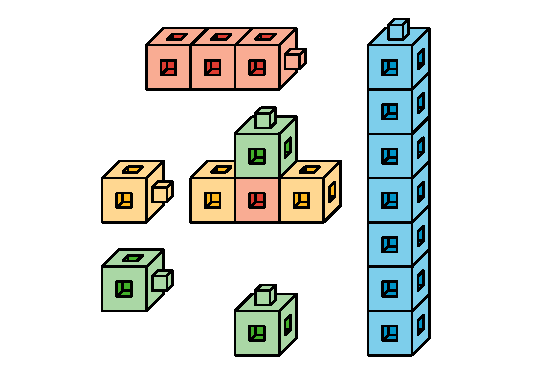
\includegraphics[width=\linewidth, center]{external/svg-source/tikz-file-147993.pdf}
\end{image}%
\end{exploration}%
\end{subsubsectionptx}
%
%
\typeout{************************************************}
\typeout{Subsubsección  Actividad 1}
\typeout{************************************************}
%
% \begin{subsubsectionptx}{Subsubsección}{Actividad 1}{}{Actividad 1}{}{}{lec-explorarCubosEncajables-act1}
% \begin{activity}{Actividad}{Conozcamos\\“Cubos encajables: Explora”.}{act-conozcamos-CubosEncajables-Explora}%
% ¡A explorar!%
% \end{activity}%
% \end{subsubsectionptx}
\end{subsectionptx}
%
%
\typeout{************************************************}
\typeout{Subsección  Lección 2 -~Exploremos las fichas geométricas}
\typeout{************************************************}
%
\begin{subsectionptx}{Subsección}{{\normalsize Lección 2\\[-0.05cm]}Exploremos las fichas geométricas}{}{Lección 2}{}{}{lec-exploremosFichasGeometricas}
\begin{introduction}{}%
Exploremos las fichas geométricas.%
\end{introduction}%
%
%
\typeout{************************************************}
\typeout{Subsubsección  Calentamiento}
\typeout{************************************************}
%
\begin{subsubsectionptx}{Subsubsección}{Calentamiento}{}{Calentamiento}{}{}{lec-exploremosFichasGeometricas-warm}
\begin{exploration}{Calentamiento}{Observa y pregúntate: Fichas geométricas.}{warm-observa-fichasGeometricas}%
¿Qué observas?\\
 ¿Qué te preguntas?%
\begin{image}{0}{1}{0}{}%
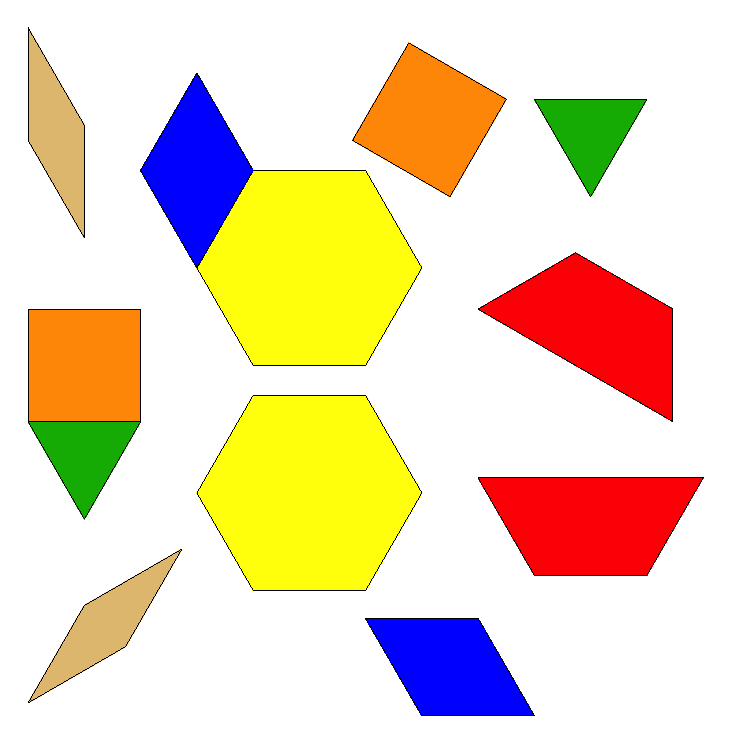
\includegraphics[max width=0.65\linewidth, center]{external/svg-source/tikz-file-148141.pdf}
\end{image}%
\end{exploration}%
\end{subsubsectionptx}
%
%
\typeout{************************************************}
\typeout{Subsubsección  Actividad 1}
\typeout{************************************************}
%
% \begin{subsubsectionptx}{Subsubsección}{Actividad 1}{}{Actividad 1}{}{}{lec-exploremosFichasGeometricas-act1}
% \begin{activity}{Actividad}{Conozcamos\\"Fichas geométricas: Explora".}{act-conozcamos-fichasGeometricas-explora}%
% ¡A explorar!%
% \end{activity}%
% \end{subsubsectionptx}
\end{subsectionptx}
%
%
\typeout{************************************************}
\typeout{Subsección  Lección 3 -~Exploremos las fichas de dos colores y los tableros de 5}
\typeout{************************************************}
%
\begin{subsectionptx}{Subsección}{{\normalsize Lección 3\\[-0.05cm]}Exploremos las fichas de dos colores y los tableros de 5}{}{Lección 3}{}{}{lec-exploremosFichasDosColoresYTableros5}
% \begin{introduction}{}%
% Exploremos las fichas de dos colores y los tableros de 5.%
% \end{introduction}%
%
%
\typeout{************************************************}
\typeout{Subsubsección  Calentamiento}
\typeout{************************************************}
%
\begin{subsubsectionptx}{Subsubsección}{Calentamiento}{}{Calentamiento}{}{}{lec-exploremosFichasDosColoresYTableros5-warm}
\begin{exploration}{Calentamiento}{Observa y pregúntate: fichas y tableros de 5.}{warm-observa-fichasYTableros5}%
¿Qué observas?\\
 ¿Qué te preguntas?%
\begin{sidebyside}{2}{0.05}{0.05}{0.1}%
\begin{sbspanel}{0.4}%

\includegraphics[max width=\linewidth, center]{external/svg-source/tikz-file-147345.pdf}
\end{sbspanel}%
\begin{sbspanel}{0.4}%
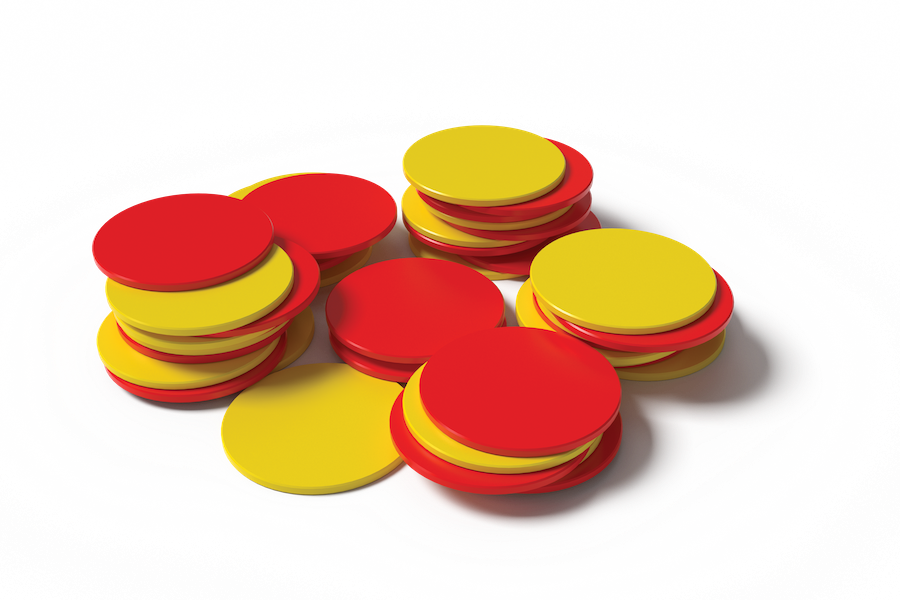
\includegraphics[max width=\linewidth, center]{external/png-source/K.1.A Beta Student Workbook.RedYellowChips_withShadow.png}
\end{sbspanel}%
\end{sidebyside}%
\begin{sidebyside}{2}{0.05}{0.05}{0.1}%
\begin{sbspanel}{0.4}%
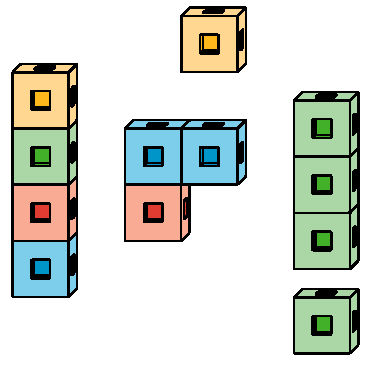
\includegraphics[max width=\linewidth, center]{external/svg-source/tikz-file-128850.pdf}
\end{sbspanel}%
\begin{sbspanel}{0.4}%
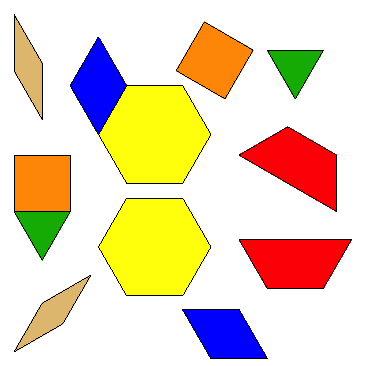
\includegraphics[max width=\linewidth, center]{external/svg-source/tikz-file-147344.pdf}
\end{sbspanel}%
\end{sidebyside}%
\end{exploration}%
\end{subsubsectionptx}
%
%
\typeout{************************************************}
\typeout{Subsubsección  Actividad 1}
\typeout{************************************************}
%
% \begin{subsubsectionptx}{Subsubsección}{Actividad 1}{}{Actividad 1}{}{}{lec-exploremosFichasDosColoresYTableros5-act1}
% \begin{activity}{Actividad}{Exploremos fichas y tableros de 5.}{act-exploremosFichasYTableros5}%
% \begin{image}{0}{1}{0}{}%
% 
\includegraphics[max width=\linewidth, center]{external/svg-source/tikz-file-148144.pdf}
% \end{image}%
% \end{activity}%
% \end{subsubsectionptx}
\end{subsectionptx}
%
%
\typeout{************************************************}
\typeout{Subsección  Lección 4 -~Exploremos los bloques sólidos geométricos}
\typeout{************************************************}
%
\begin{subsectionptx}{Subsección}{{\normalsize Lección 4\\[-0.05cm]}Exploremos los bloques sólidos geométricos}{}{Lección 4}{}{}{lec-exploremosBloquesSolidosGeom}
% \begin{introduction}{}%
% Exploremos los bloques sólidos geométricos.%
% \end{introduction}%
%
%
\typeout{************************************************}
\typeout{Subsubsección  Calentamiento}
\typeout{************************************************}
%
\begin{subsubsectionptx}{Subsubsección}{Calentamiento}{}{Calentamiento}{}{}{lec-exploremosBloquesSolidosGeom-warm}
\begin{exploration}{Calentamiento}{Observa y pregúntate: Bloques sólidos geométricos.}{warm-observa-bloquesSolidosGeom}%
¿Qué observas?\\
 ¿Qué te preguntas?%
\begin{image}{0.0}{1}{0.0}{}%
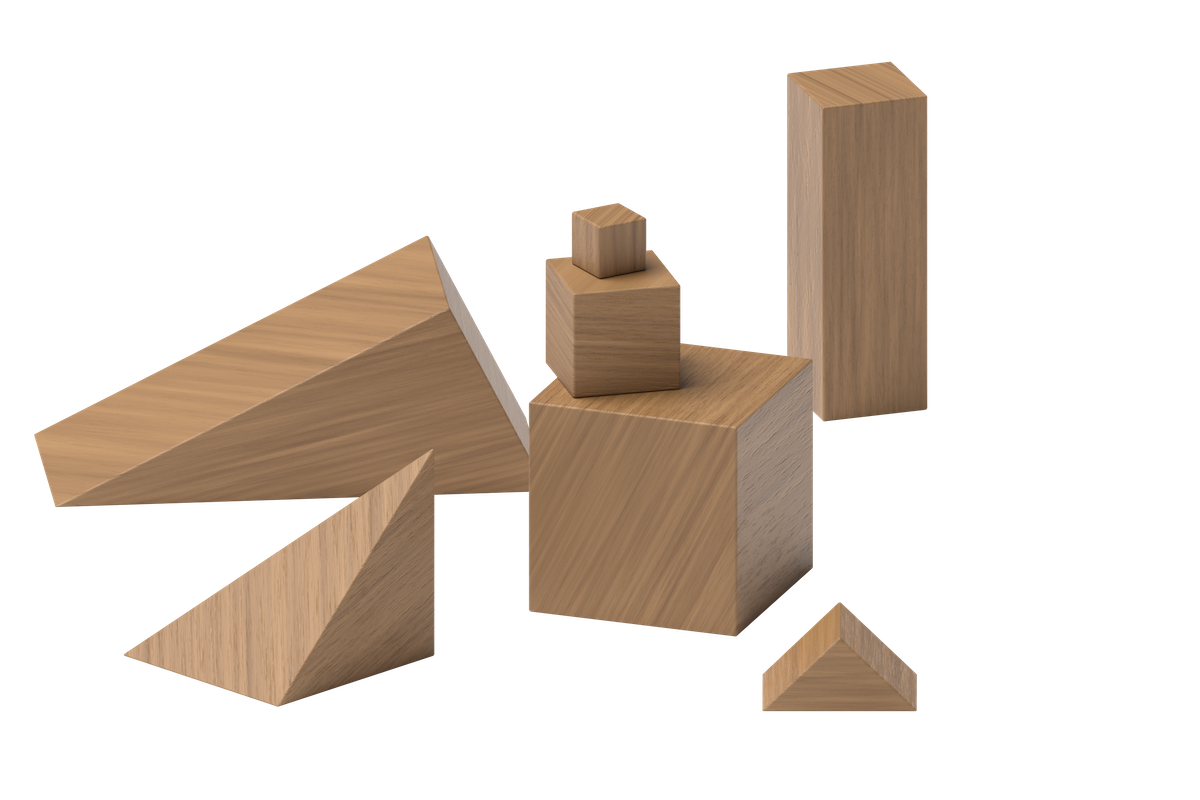
\includegraphics[max width=\linewidth, center]{external/png-source/K.1.A Beta Student Workbook.Geoblocks.png}
\end{image}%
\end{exploration}%
\end{subsubsectionptx}
%
%
\typeout{************************************************}
\typeout{Subsubsección  Actividad 1}
\typeout{************************************************}
%
% \begin{subsubsectionptx}{Subsubsección}{Actividad 1}{}{Actividad 1}{}{}{lec-exploremosBloquesSolidosGeom-act1}
% \begin{activity}{Actividad}{Conozcamos\\``Bloques sólidos geométricos: Explora''.}{act-conozcamos-bloquesSolidosGeom-explora}%
% ¡Exploremos con los bloques!%
% \end{activity}%
% \end{subsubsectionptx}
%
%
\typeout{************************************************}
\typeout{Subsubsección  Actividad 2}
\typeout{************************************************}
%
% \clearpage
\begin{subsubsectionptx}{Subsubsección}{Actividad 2}{}{Actividad 2}{}{}{lec-exploremosBloquesSolidosGeom-act2}
\begin{activity}{Actividad}{Conozcamos\\“Bloques sólidos geométricos: Construye lo que ves”.}{act-conozcamos-bloquesSolidosGeom-construyeVes}%
Usa bloques para construir una casa.%
\begin{image}{0}{1}{0}{}%
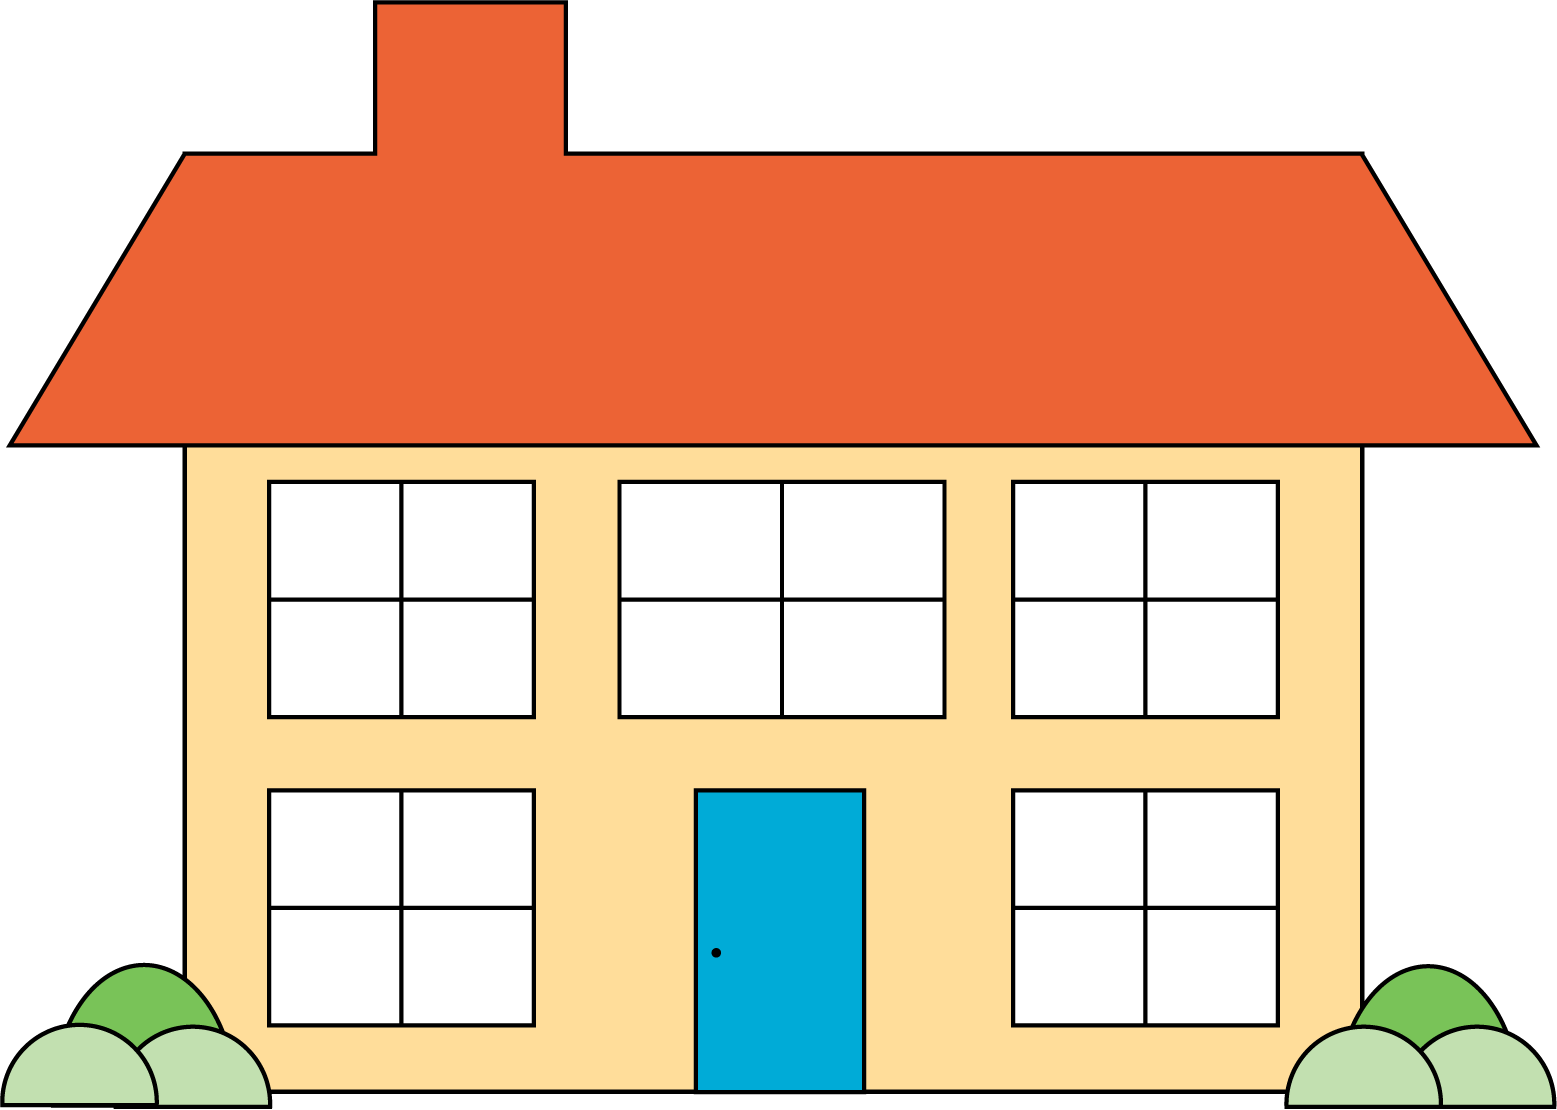
\includegraphics[width=\linewidth, center]{external/png-source/house.png}
\end{image}%
\end{activity}%
\end{subsubsectionptx}
\end{subsectionptx}
%
%
\typeout{************************************************}
\typeout{Subsección  Lección 5 -~Exploremos nuestras herramientas matemáticas}
\typeout{************************************************}
%
\begin{subsectionptx}{Subsección}{{\normalsize Lección 5\\[-0.05cm]}Exploremos nuestras herramientas matemáticas}{}{Lección 5}{}{}{lec-exploremosHerramientasMate}
\begin{introduction}{}%
Exploremos nuestras herramientas matemáticas.%
\end{introduction}%
%
%
\typeout{************************************************}
\typeout{Subsubsección  Calentamiento}
\typeout{************************************************}
%
\begin{subsubsectionptx}{Subsubsección}{Calentamiento}{}{Calentamiento}{}{}{lec-exploremosHerramientasMate-warm}
\begin{exploration}{Calentamiento}{Observa y pregúntate: Usa herramientas distintas.}{warm-observa-herramientasDistintas}%
¿Qué observas?\\
 ¿Qué te preguntas?%
\begin{sidebyside}{2}{0.05}{0.05}{0.1}%
\begin{sbspanel}{0.4}%
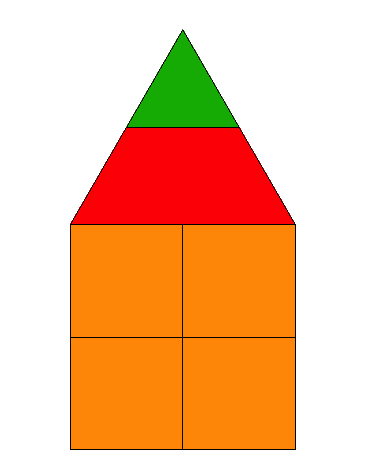
\includegraphics[max width=\linewidth, center]{external/svg-source/tikz-file-148145.pdf}
\end{sbspanel}%
\begin{sbspanel}{0.4}%
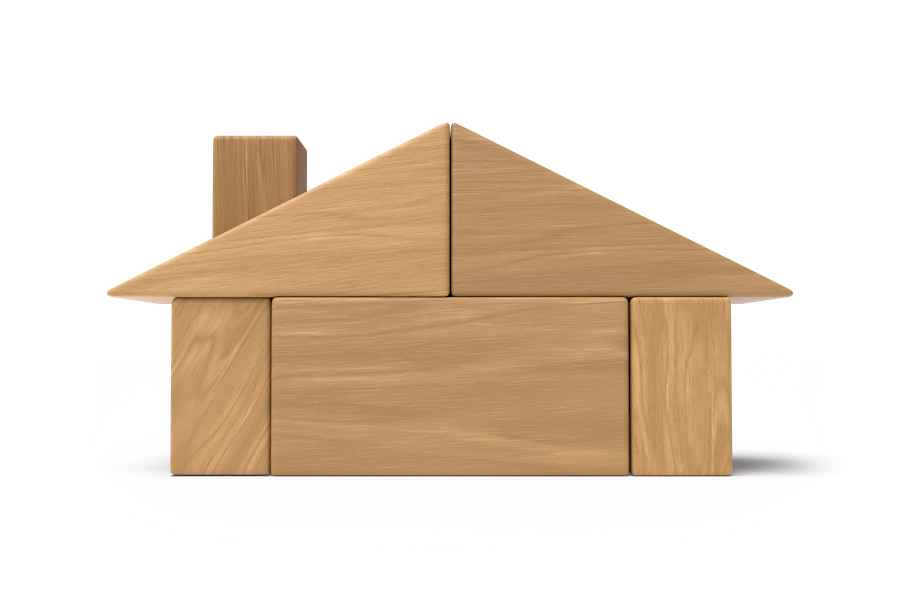
\includegraphics[max width=\linewidth, center]{external/png-source/K.1.A Beta Student Workbook.Woodhouse_withShadow.png}
\par
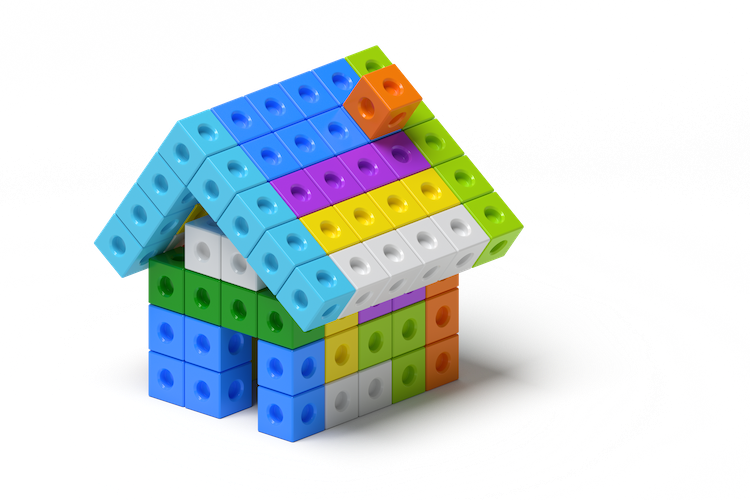
\includegraphics[max width=\linewidth, center]{external/png-source/5.1.A2.House_withShadow.png}
\end{sbspanel}%
\end{sidebyside}%
\end{exploration}%
\end{subsubsectionptx}
%
%
\typeout{************************************************}
\typeout{Subsubsección  Actividad 1}
\typeout{************************************************}
%
% \begin{multicols}{2}
\begin{subsubsectionptx}{Subsubsección}{Actividad 1}{}{Actividad 1}{}{}{lec-exploremosHerramientasMate-act1}
\begin{activity}{Actividad}{Conozcamos\\“Cubos encajables: Construye lo que ves”.}{act-conozcamos-construyeLoQueVes}%
\begin{image}{0}{1}{0}{}%
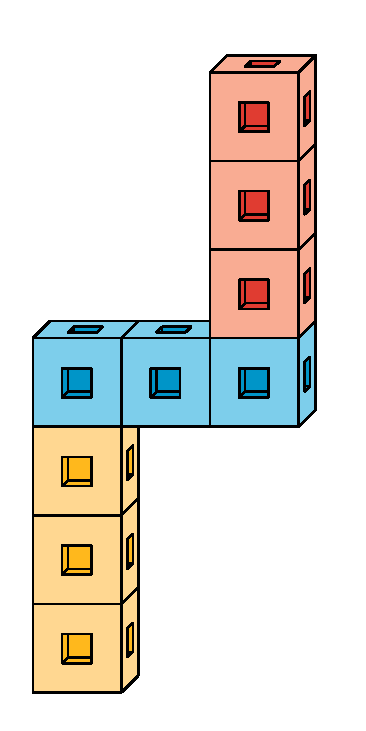
\includegraphics[ width=0.26\linewidth, center]{external/svg-source/tikz-file-148146.pdf}
\end{image}%
\end{activity}%
\end{subsubsectionptx}
%
%
\typeout{************************************************}
\typeout{Subsubsección  Actividad 2}
\typeout{************************************************}
%
\begin{subsubsectionptx}{Subsubsección}{Actividad 2}{}{Actividad 2}{}{}{lec-exploremosHerramientasMate-act2}
\begin{activity}{Actividad}{Conozcamos\\“Fichas geométricas: Rompecabezas”.}{act-conozcamos-fichasGeometricas-rompecabezas}%
\begin{image}{0}{1}{0}{}%

\includegraphics[width=0.5\linewidth, center]{external/svg-source/tikz-file-148147.pdf}
\end{image}%
\end{activity}%
\end{subsubsectionptx}
% \end{multicols}
%
%
\typeout{************************************************}
\typeout{Subsubsección  Actividad 3}
\typeout{************************************************}
%
\clearpage
\begin{subsubsectionptx}{Subsubsección}{Actividad 3}{}{Actividad 3}{}{}{lec-exploremosHerramientasMate-act3}
\begin{activity}{Actividad}{Centros: Momento de escoger.}{act-centros-escoger1}%
Escoge un centro.%
\begin{sidebyside}{2}{0.05}{0.05}{0.1}%
\begin{sbspanel}{0.5}[center]%
Bloques sólidos geométricos%
\end{sbspanel}%
\begin{sbspanel}{0.3}[center]%
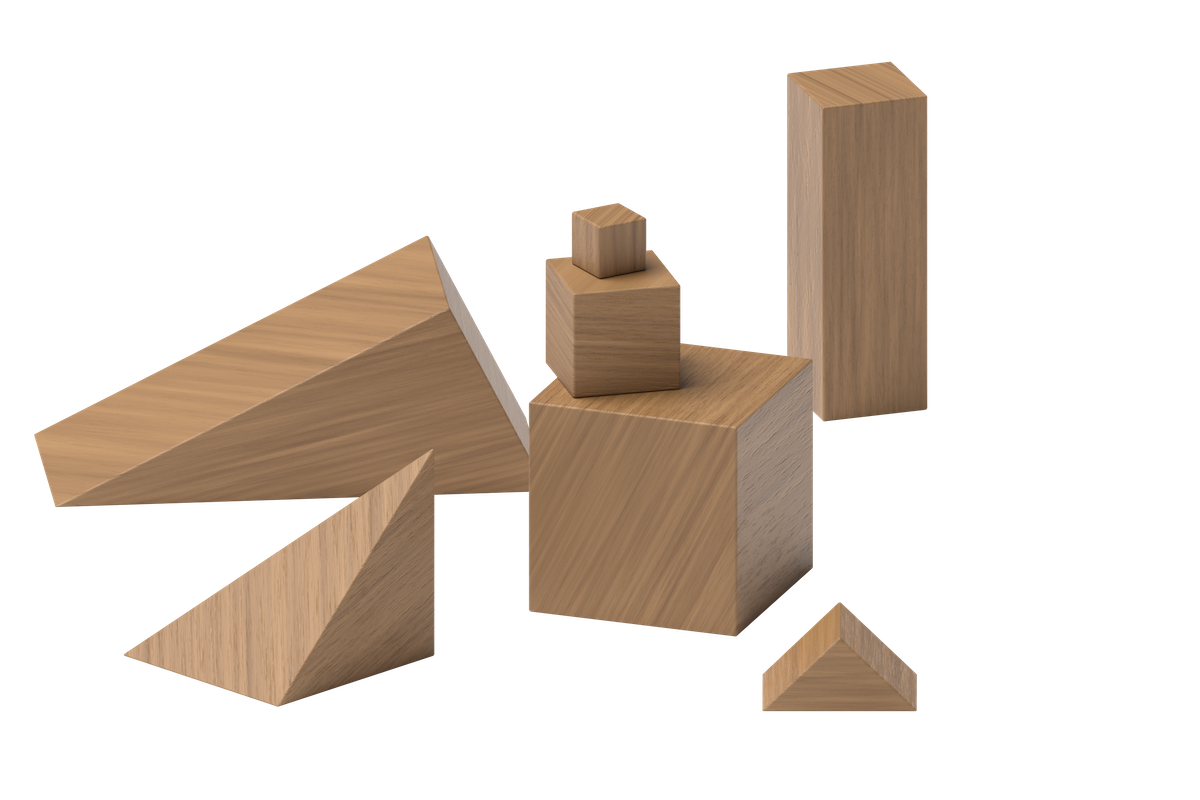
\includegraphics[max width=\linewidth, center]{external/png-source/K.1.A Beta Student Workbook.Geoblocks.png}
\end{sbspanel}%
\end{sidebyside}%
\begin{sidebyside}{2}{0.05}{0.05}{0.1}%
\begin{sbspanel}{0.5}[center]%
Cubos encajables%
\end{sbspanel}%
\begin{sbspanel}{0.3}[center]%
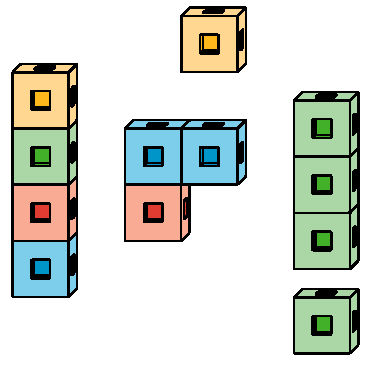
\includegraphics[max width=\linewidth, center]{external/svg-source/tikz-file-128850.pdf}
\end{sbspanel}%
\end{sidebyside}%
\begin{sidebyside}{2}{0.05}{0.05}{0.1}%
\begin{sbspanel}{0.5}[center]%
Fichas geométricas%
\end{sbspanel}%
\begin{sbspanel}{0.3}[center]%
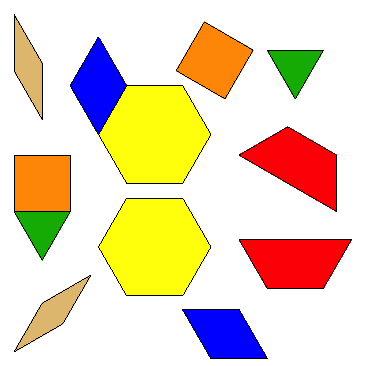
\includegraphics[max width=\linewidth, center]{external/svg-source/tikz-file-147344.pdf}
\end{sbspanel}%
\end{sidebyside}%
\end{activity}%
\end{subsubsectionptx}
\end{subsectionptx}
%
%
\typeout{************************************************}
\typeout{Referencias  Resumen de la sección}
\typeout{************************************************}
%
\begin{references-subsection}{Referencias}{Resumen de la sección}{}{Resumen sección}{}{}{gra0-uni1-secA-resumen}
Exploramos muchas herramientas matemáticas.%
\begin{sidebyside}{2}{0.05}{0.05}{0.1}%
\begin{sbspanel}{0.4}%
Cubos Encajables%
\par
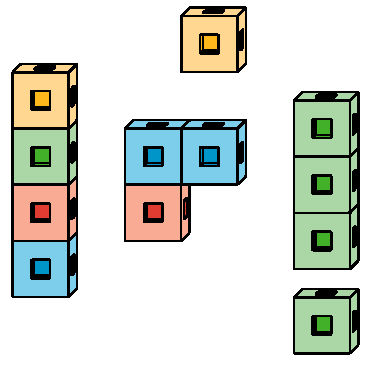
\includegraphics[max width=\linewidth, center]{external/svg-source/tikz-file-128850.pdf}
\end{sbspanel}%
\begin{sbspanel}{0.4}%
Fichas Geométricas%
\par
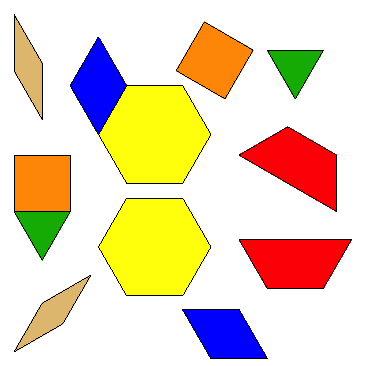
\includegraphics[max width=\linewidth, center]{external/svg-source/tikz-file-147344.pdf}
\end{sbspanel}%
\end{sidebyside}%
\begin{sidebyside}{2}{0.05}{0.05}{0.1}%
\begin{sbspanel}{0.4}%
Bloques sólidos geométricos%
\par
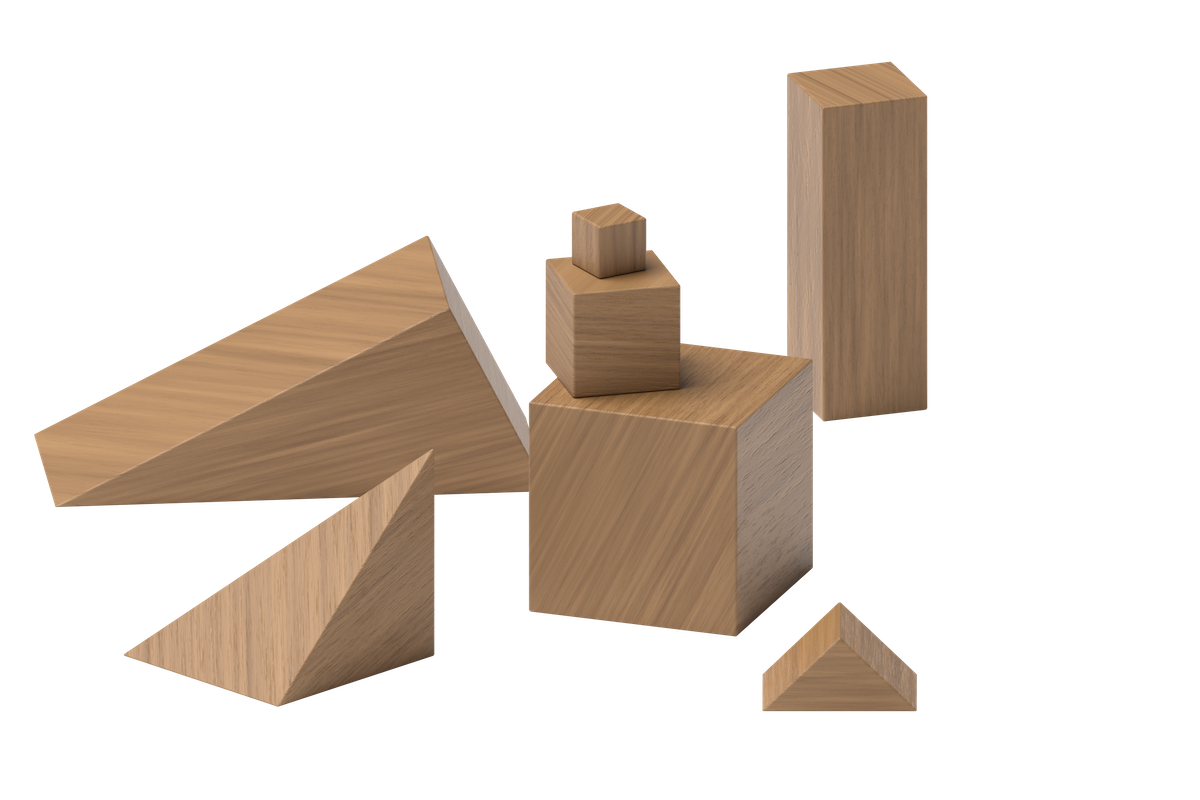
\includegraphics[max width=\linewidth, center]{external/png-source/K.1.A Beta Student Workbook.Geoblocks.png}
\end{sbspanel}%
\begin{sbspanel}{0.4}%
Fichas de dos colores%
\par
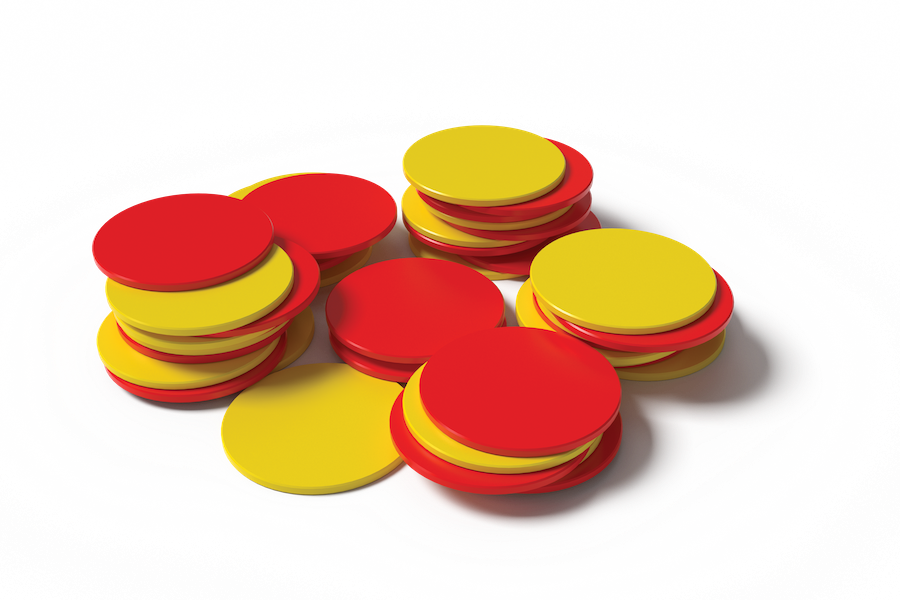
\includegraphics[max width=\linewidth, center]{external/png-source/K.1.A Beta Student Workbook.RedYellowChips_withShadow.png}
\end{sbspanel}%
\end{sidebyside}%
\begin{sidebyside}{2}{0.05}{0.05}{0.1}%
\begin{sbspanel}{0.4}%
Tableros de 5%
\par

\includegraphics[max width=\linewidth, center]{external/svg-source/tikz-file-148144.pdf}
\end{sbspanel}%
\begin{sbspanel}{0.4}%
%
\end{sbspanel}%
\end{sidebyside}%
\end{references-subsection}
\end{sectionptx}
%
%
\typeout{************************************************}
\typeout{Sección  Sección B -~Reconozcamos cantidades}
\typeout{************************************************}
%
\begin{sectionptx}{Sección}{{\Large Sección B\\}Reconozcamos cantidades}{}{Sección B -~Reconozcamos cantidades}{}{}{gra0-uni1-secB}
%
%
\typeout{************************************************}
\typeout{Subsección  Lección 6 -~Busquemos grupos pequeños}
\typeout{************************************************}
%
\begin{subsectionptx}{Subsección}{{\normalsize Lección 6\\[-0.05cm]}Busquemos grupos pequeños}{}{Lección 6}{}{}{lec-busquemosGruposMasPequenos}
\begin{introduction}{}%
Busquemos grupos pequeños de objetos.%
\end{introduction}%
%
%
\typeout{************************************************}
\typeout{Subsubsección  Calentamiento}
\typeout{************************************************}
%
\begin{subsubsectionptx}{Subsubsección}{Calentamiento}{}{Calentamiento}{}{}{lec-busquemosGruposMasPequenos-warm}
\begin{exploration}{Calentamiento}{Actuémoslo: Introducción.}{warm-actuemoslo-intro}%
\begin{image}{0.1}{0.8}{0.1}{}%

\includegraphics[max width=\linewidth, center]{external/png-source/3 ducks.png}
\end{image}%
\par
\vspace*{2ex}
3 patitos muy lejos de aquí\\
 a la colina salieron a pasear.\\
 Mamá pata dijo: “Cuac, cuac, cuac”.\\
 Después 3 patitos vio regresar.%
\end{exploration}%
\end{subsubsectionptx}
%
%
\typeout{************************************************}
\typeout{Subsubsección  Actividad 1}
\typeout{************************************************}
%
% \clearpage
\begin{subsubsectionptx}{Subsubsección}{Actividad 1}{}{Actividad 1}{}{}{lec-busquemosGruposMasPequenos-act1}
\begin{activity}{Actividad}{Cuántos ves: Introducción.}{act-cuantosVes-intro}%
\begin{minipage}{0.6\linewidth}
¿Cuántos ves?\\
 ¿Cómo lo sabes?, ¿qué ves?%
\end{minipage}
\hfill
\begin{minipage}{0.3\linewidth}
\begin{image}{0}{1}{0}{}%

\includegraphics[max width=\linewidth, center]{external/svg-source/tikz-file-148150.pdf}
\end{image}%
\end{minipage}
% \end{multicols}
\end{activity}%
\end{subsubsectionptx}
%
%
\typeout{************************************************}
\typeout{Subsubsección  Actividad 2}
\typeout{************************************************}
%
% \clearpage
% \begin{subsubsectionptx}{Subsubsección}{Actividad 2}{}{Actividad 2}{}{}{lec-busquemosGruposMasPequenos-act2}
% \begin{activity}{Actividad}{Conozcamos\\“Libros de imágenes: Explora”.}{act-conozcamos-librosDeImagenes-explora}%
% Busquen grupos de cosas en su libro.%
% \end{activity}%
% \end{subsubsectionptx}
%
%
\typeout{************************************************}
\typeout{Subsubsección  Actividad 3}
\typeout{************************************************}
%
\clearpage
\begin{subsubsectionptx}{Subsubsección}{Actividad 3}{}{Actividad 3}{}{}{lec-busquemosGruposMasPequenos-act3}
\begin{activity}{Actividad}{Centros: Momento de escoger.}{act-centros-escoger2}%
\begin{sidebyside}{2}{0.025}{0.025}{0.05}%
\begin{sbspanel}{0.45}%
Cubos Encajables%
\par
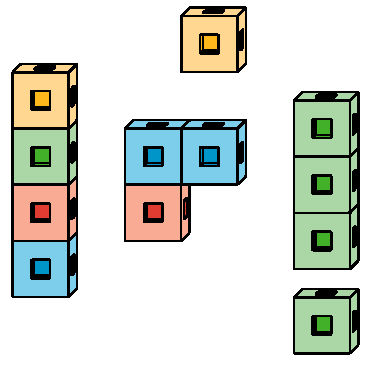
\includegraphics[max width=\linewidth, center]{external/svg-source/tikz-file-128850.pdf}
\end{sbspanel}%
\begin{sbspanel}{0.45}%
Fichas Geométricas%
\par
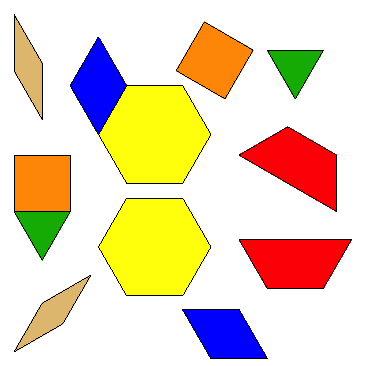
\includegraphics[max width=\linewidth, center]{external/svg-source/tikz-file-147344.pdf}
\end{sbspanel}%
\end{sidebyside}%
\vspace*{1ex minus 0.8ex}
\begin{sidebyside}{2}{0.025}{0.025}{0.05}%
\begin{sbspanel}{0.45}%
Bloques sólidos geométricos%
\par
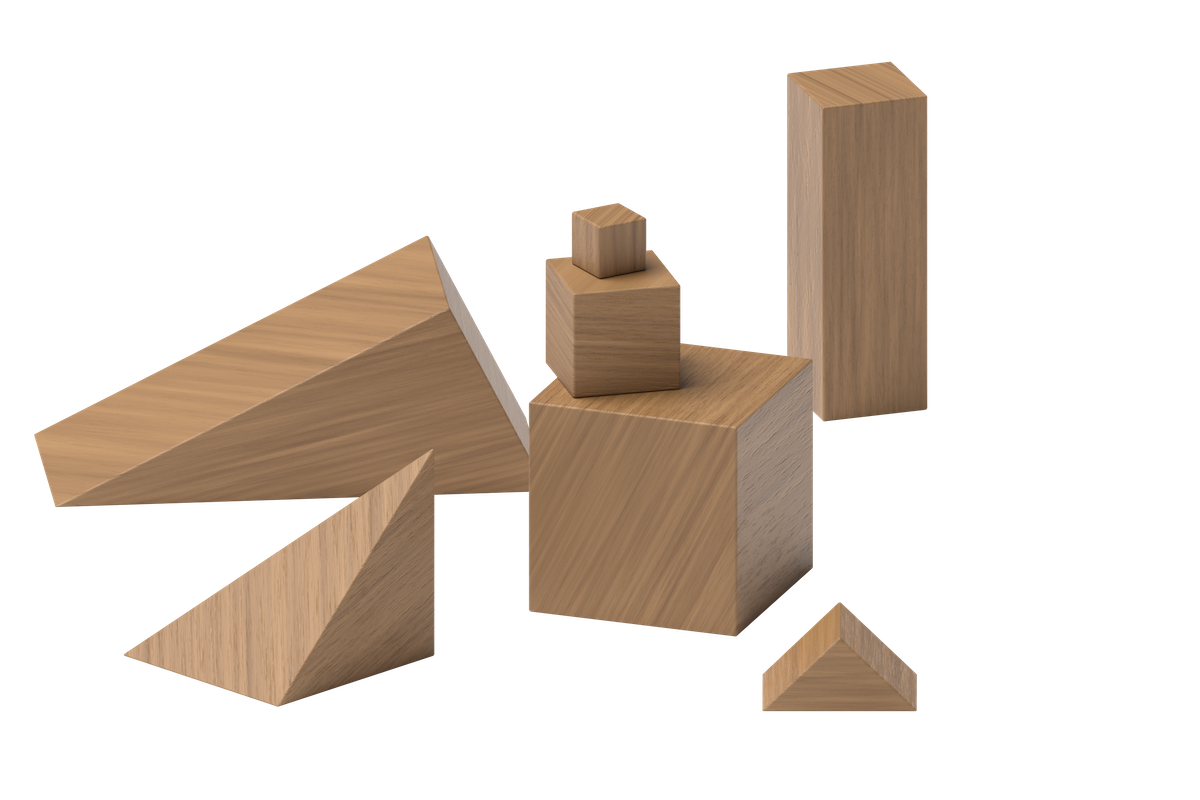
\includegraphics[max width=\linewidth, center]{external/png-source/K.1.A Beta Student Workbook.Geoblocks.png}
\end{sbspanel}%
\begin{sbspanel}{0.45}%
Libros de imágenes%
\par

\includegraphics[max width=\linewidth, center]{external/png-source/K.1.D Beta Student Workbooks.Books.png}
\end{sbspanel}%
\end{sidebyside}%
\end{activity}%
\end{subsubsectionptx}
\end{subsectionptx}
%
%
\typeout{************************************************}
\typeout{Subsección  Lección 7 -~Juego de búsqueda en el salón de clase}
\typeout{************************************************}
%
\begin{subsectionptx}{Subsección}{{\normalsize Lección 7\\[-0.05cm]}Juego de búsqueda en el salón de clase}{}{Lección 7}{}{}{lec-juegoBusqueda}
\begin{introduction}{}%
Busquemos grupos de objetos en el salón de clase.%
\end{introduction}%
%
%
\typeout{************************************************}
\typeout{Subsubsección  Calentamiento}
\typeout{************************************************}
%
\begin{subsubsectionptx}{Subsubsección}{Calentamiento}{}{Calentamiento}{}{}{lec-juegoBusqueda-warm}
\begin{exploration}{Calentamiento}{¿Cómo lo podemos mostrar?}{warm-comoPodemosMostrar}%
\begin{image}{0.0}{1}{0.0}{}%

\includegraphics[max width=\linewidth, center]{external/png-source/3 ducks.png}
\end{image}%
%
\par
\vspace*{2ex}
3 patitos muy lejos de aqui\\
 a la colina salieron a pasear.\\
 Mamá pata dijo: “Cuac, cuac, cuac”.\\
 Después 3 patitos vio regresar.%
\end{exploration}%
\end{subsubsectionptx}
%
%
\typeout{************************************************}
\typeout{Subsubsección  Actividad 1}
\typeout{************************************************}
%
\clearpage
\begin{subsubsectionptx}{Subsubsección}{Actividad 1}{}{Actividad 1}{}{}{lec-juegoBusqueda-act1}
\begin{activity}{Actividad}{Cuántos ves: Dos imágenes.}{act-cuantosVes-imagenes}%
¿Cuántos ves?\\
 ¿Cómo lo sabes?, ¿qué ves?%
\begin{sidebyside}{2}{0}{0}{0}%
\begin{sbspanel}{0.5}%

\includegraphics[max width=\linewidth, center]{external/svg-source/tikz-file-148152.pdf}
\end{sbspanel}%
\begin{sbspanel}{0.5}%

\includegraphics[max width=\linewidth, center]{external/svg-source/tikz-file-148153.pdf}
\end{sbspanel}%
\end{sidebyside}%
\end{activity}%
\end{subsubsectionptx}
%
%
\typeout{************************************************}
\typeout{Subsubsección  Actividad 2}
\typeout{************************************************}
%
\begin{subsubsectionptx}{Subsubsección}{Actividad 2}{}{Actividad 2}{}{}{lec-juegoBusqueda-act2}
\begin{activity}{Actividad}{Juego de búsqueda en el salón de clase.}{act-juegoBusqueda}%
Busca 3 objetos en nuestro salón.%
\end{activity}%
\end{subsubsectionptx}
%
%
\typeout{************************************************}
\typeout{Subsubsección  Actividad 3}
\typeout{************************************************}
%
\clearpage
\begin{subsubsectionptx}{Subsubsección}{Actividad 3}{}{Actividad 3}{}{}{lec-juegoBusqueda-act3}
\begin{activity}{Actividad}{Centros: Momento de escoger.}{act-centros-escoger3}%
Escoge un centro.%
\begin{sidebyside}{2}{0.025}{0.025}{0.05}%
\begin{sbspanel}{0.45}%
Cubos Encajables%
\par
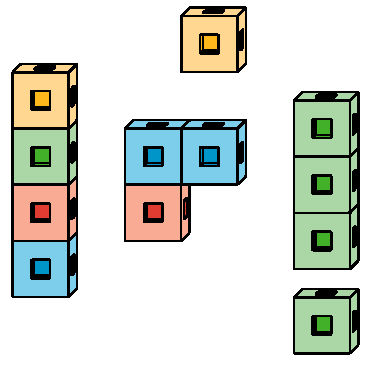
\includegraphics[max width=\linewidth, center]{external/svg-source/tikz-file-128850.pdf}
\end{sbspanel}%
\begin{sbspanel}{0.45}%
Fichas Geométricas%
\par
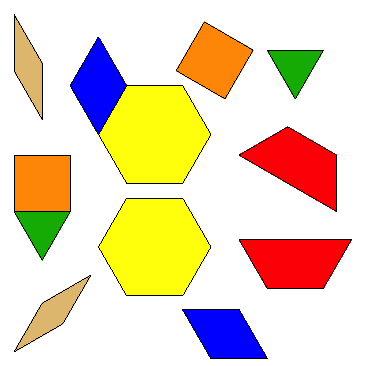
\includegraphics[max width=\linewidth, center]{external/svg-source/tikz-file-147344.pdf}
\end{sbspanel}%
\end{sidebyside}%
\vspace*{1ex minus 0.8ex}
\begin{sidebyside}{2}{0.025}{0.025}{0.05}%
\begin{sbspanel}{0.45}%
Bloques sólidos geométricos%
\par
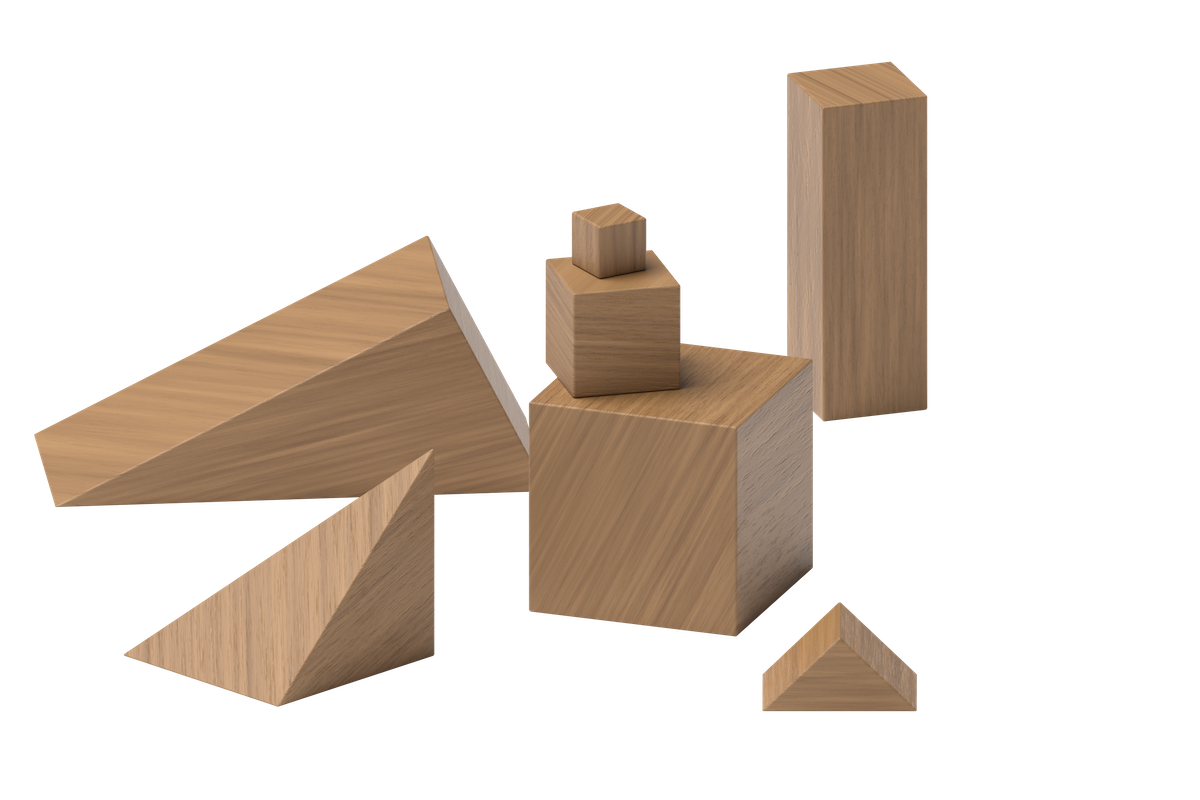
\includegraphics[max width=\linewidth, center]{external/png-source/K.1.A Beta Student Workbook.Geoblocks.png}
\end{sbspanel}%
\begin{sbspanel}{0.45}%
Libros de imágenes%
\par

\includegraphics[max width=\linewidth, center]{external/png-source/K.1.D Beta Student Workbooks.Books.png}
\end{sbspanel}%
\end{sidebyside}%
\end{activity}%
\end{subsubsectionptx}
\end{subsectionptx}
%
%
\typeout{************************************************}
\typeout{Subsección  Lección 8 -~Grupos diferentes, misma cantidad}
\typeout{************************************************}
%
\begin{subsectionptx}{Subsección}{{\normalsize Lección 8\\[-0.05cm]}Grupos diferentes, misma cantidad}{}{Lección 8}{}{}{lec-gruposDiferentesMismaCantidad}
\begin{introduction}{}%
Encontremos grupos que tengan el mismo número de cosas.%
\end{introduction}%
%
%
\typeout{************************************************}
\typeout{Subsubsección  Calentamiento}
\typeout{************************************************}
%
\begin{subsubsectionptx}{Subsubsección}{Calentamiento}{}{Calentamiento}{}{}{lec-gruposDiferentesMismaCantidad-warm}
\begin{exploration}{Calentamiento}{Actuémoslo: Otra manera.}{warm-actuemoslo-otraManera}%
\begin{image}{0.0}{1}{0.0}{}%

\includegraphics[max width=\linewidth, center]{external/png-source/3 ducks.png}
\end{image}%
%
\par
\vspace*{2ex}
3 patitos muy lejos de aquí\\
 a la colina salieron a pasear.\\
 Mamá pata dijo: “Cuac, cuac, cuac.”\\
 Después 3 patitos vio regresar.%
\end{exploration}%
\end{subsubsectionptx}
%
%
\typeout{************************************************}
\typeout{Subsubsección  Actividad 1}
\typeout{************************************************}
%
\clearpage
\begin{subsubsectionptx}{Subsubsección}{Actividad 1}{}{Actividad 1}{}{}{lec-gruposDiferentesMismaCantidad-act1}
\begin{activity}{Actividad}{Cuántos ves: 1, 2, 3.}{act-cuantosVes-123}%
¿Cuántos ves?\\
 ¿Cómo lo sabes?, ¿qué ves?%
\begin{sidebyside}{3}{0.0416666666666667}{0.0416666666666667}{0.0833333333333333}%
\begin{sbspanel}{0.25}%

\includegraphics[max width=\linewidth, center]{external/svg-source/tikz-file-136322.pdf}
\end{sbspanel}%
\begin{sbspanel}{0.25}%

\includegraphics[max width=\linewidth, center]{external/svg-source/tikz-file-136323.pdf}
\end{sbspanel}%
\begin{sbspanel}{0.25}%

\includegraphics[max width=\linewidth, center]{external/svg-source/tikz-file-136324.pdf}
\end{sbspanel}%
\end{sidebyside}%
\end{activity}%
\end{subsubsectionptx}
%
%
\typeout{************************************************}
\typeout{Subsubsección  Actividad 2}
\typeout{************************************************}
%
\begin{subsubsectionptx}{Subsubsección}{Actividad 2}{}{Actividad 2}{}{}{lec-gruposDiferentesMismaCantidad-act2}
\begin{activity}{Actividad}{Grupos diferentes, misma cantidad.}{act-gruposDiferentesMismaCantidad}%
\begin{image}{0}{1}{0}{}%
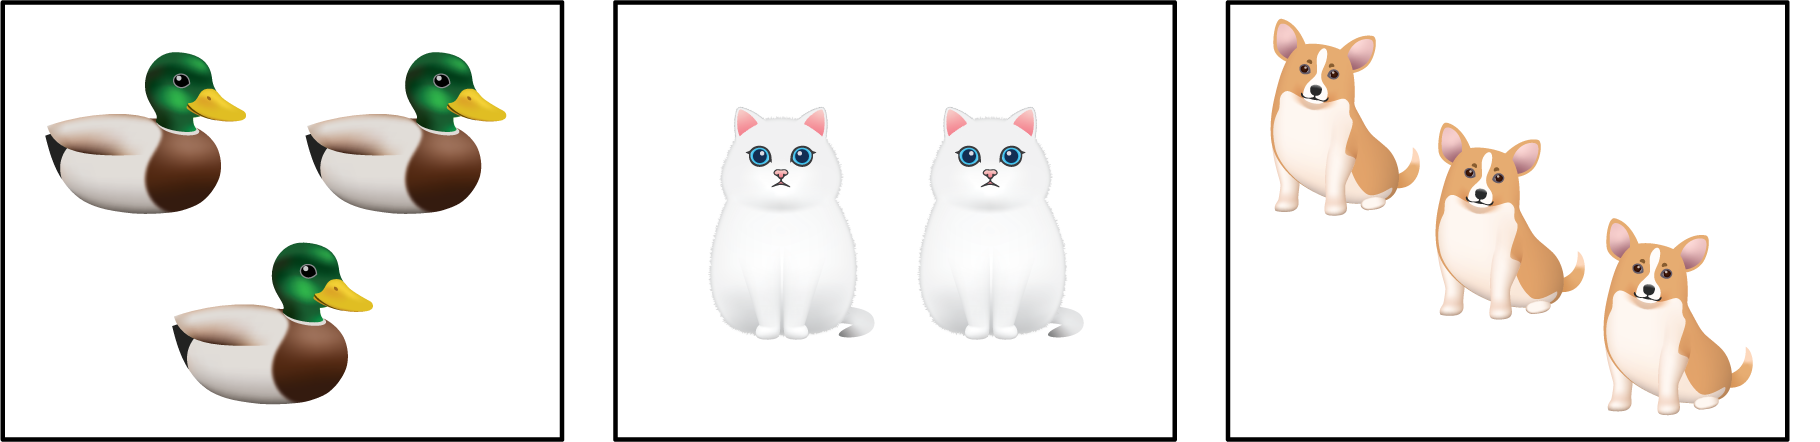
\includegraphics[max width=\linewidth, center]{external/png-source/K.1.C Beta Student Workbook.AnimalGroups.png}
\end{image}%
%
\end{activity}%
\end{subsubsectionptx}
%
%
\typeout{************************************************}
\typeout{Subsubsección  Actividad 3}
\typeout{************************************************}
%
\clearpage
\begin{subsubsectionptx}{Subsubsección}{Actividad 3}{}{Actividad 3}{}{}{lec-gruposDiferentesMismaCantidad-act3}
\begin{activity}{Actividad}{Centros: Momento de escoger.}{act-centros-escoger4}%
Escoge un centro.%
\begin{sidebyside}{2}{0.025}{0.025}{0.05}%
\begin{sbspanel}{0.45}%
Cubos Encajables%
\par
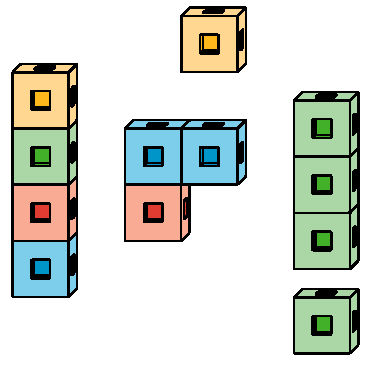
\includegraphics[max width=\linewidth, center]{external/svg-source/tikz-file-128850.pdf}
\end{sbspanel}%
\begin{sbspanel}{0.45}%
Fichas Geométricas%
\par
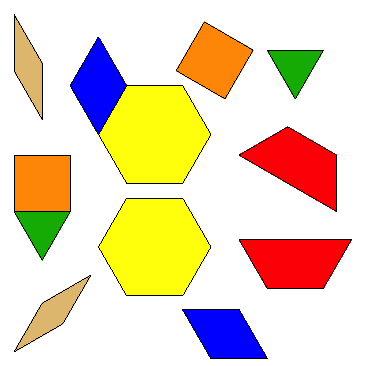
\includegraphics[max width=\linewidth, center]{external/svg-source/tikz-file-147344.pdf}
\end{sbspanel}%
\end{sidebyside}%
\vspace*{1ex minus 0.8ex}
\begin{sidebyside}{2}{0.025}{0.025}{0.05}%
\begin{sbspanel}{0.45}%
Bloques sólidos geométricos%
\par
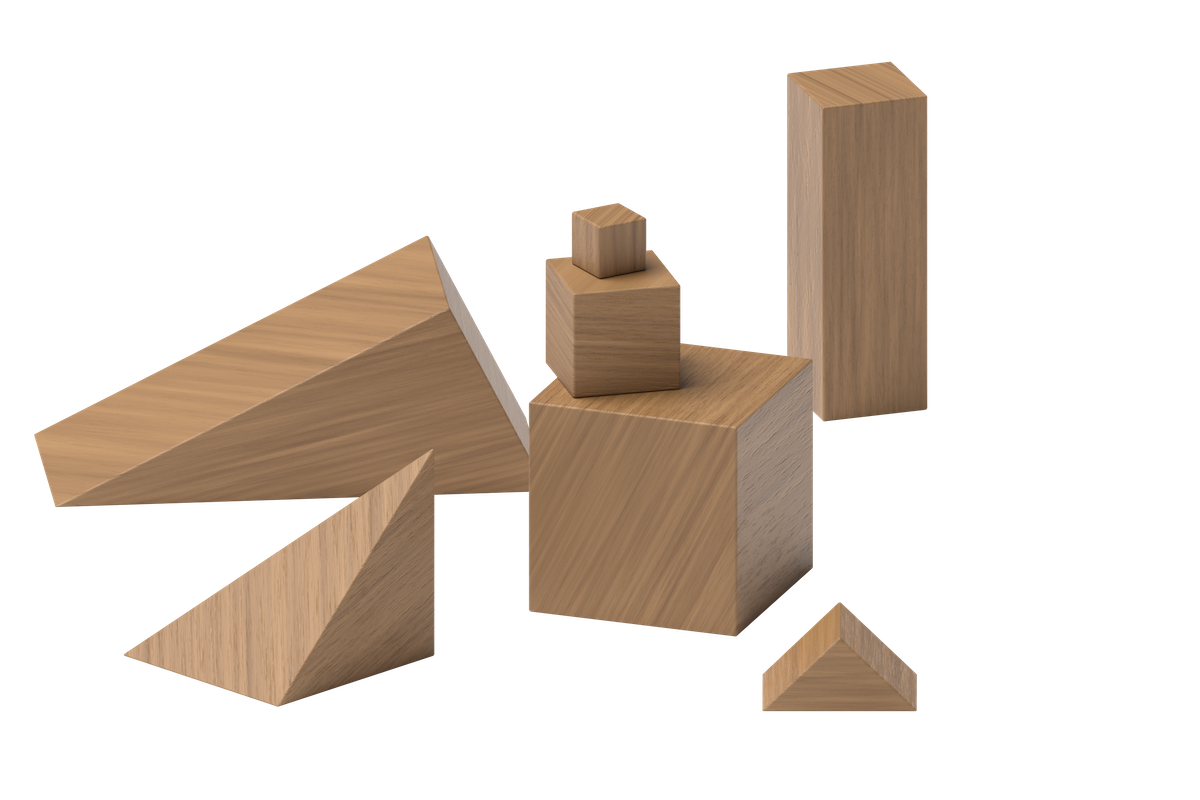
\includegraphics[max width=\linewidth, center]{external/png-source/K.1.A Beta Student Workbook.Geoblocks.png}
\end{sbspanel}%
\begin{sbspanel}{0.45}%
Libros de imágenes%
\par

\includegraphics[max width=\linewidth, center]{external/png-source/K.1.D Beta Student Workbooks.Books.png}
\end{sbspanel}%
\end{sidebyside}%
\end{activity}%
\end{subsubsectionptx}
\end{subsectionptx}
%
%
\typeout{************************************************}
\typeout{Subsección  Lección 9 -~Hagamos libros de imágenes}
\typeout{************************************************}
%
\begin{subsectionptx}{Subsección}{{\normalsize Lección 9\\[-0.05cm]}Hagamos libros de imágenes}{}{Lección 9}{}{}{lec-hagamosDeLibrosImagenes}
\begin{introduction}{}%
Hagamos libros de imágenes acerca de nuestro salón de clase.%
\end{introduction}%
%
%
\typeout{************************************************}
\typeout{Subsubsección  Calentamiento}
\typeout{************************************************}
%
\begin{subsubsectionptx}{Subsubsección}{Calentamiento}{}{Calentamiento}{}{}{lec-hagamosDeLibrosImagenes-warm}
\begin{exploration}{Calentamiento}{Actuémoslo: La historia cambia.}{warm-actuemoslo-laHistoriaCambia}%
\begin{image}{0.0}{1}{0.0}{}%

\includegraphics[max width=\linewidth, center]{external/png-source/3 ducks.png}
\end{image}%
%
\par
\vspace*{2ex}
3 patitos muy lejos de aquí\\
 a la colina salieron a pasear.\\
 Mamá pata dijo: “Cuac, cuac, cuac.”\\
 Después 3 patitos vio regresar.%
\par
3 patitos muy lejos de aquí\\
 a la colina salieron a pasear.\\
 Mamá pata dijo: “Cuac, cuac, cuac.”\\
 Después 2 patitos vio regresar.%
\end{exploration}%
\end{subsubsectionptx}
%
%
\typeout{************************************************}
\typeout{Subsubsección  Actividad 1}
\typeout{************************************************}
%
\clearpage
\begin{subsubsectionptx}{Subsubsección}{Actividad 1}{}{Actividad 1}{}{}{lec-hagamosDeLibrosImagenes-act1}
\begin{activity}{Actividad}{Cuántos ves: ¿Qué observas?}{act-cuantosVes-queObservas}%
¿Cuántos ves?\\
 ¿Cómo lo sabes?, ¿qué ves?%
\begin{sidebyside}{2}{0}{0}{0}%
\begin{sbspanel}{0.5}%

\includegraphics[max width=\linewidth, center]{external/svg-source/tikz-file-148154.pdf}
\end{sbspanel}%
\begin{sbspanel}{0.5}%

\includegraphics[max width=\linewidth, center]{external/svg-source/tikz-file-147348.pdf}
\end{sbspanel}%
\end{sidebyside}%
\end{activity}%
\end{subsubsectionptx}
%
%
\typeout{************************************************}
\typeout{Subsubsección  Actividad 2}
\typeout{************************************************}
%
\begin{subsubsectionptx}{Subsubsección}{Actividad 2}{}{Actividad 2}{}{}{lec-hagamosDeLibrosImagenes-act2}
\begin{activity}{Actividad}{Conozcamos\\“Libros de imágenes: Crea”.}{act-conozcamos-librosDeImagenes-crea}%
Dibuja cosas de nuestro salón de las que haya dos.%
\begin{sidebyside}{2}{0.3}{0.3}{0}%
\begin{sbspanel}{0.2}%

\includegraphics[max width=\linewidth, center]{external/svg-source/tikz-file-148155.pdf}
\end{sbspanel}%
\begin{sbspanel}{0.2}%

\includegraphics[max width=\linewidth, center]{external/svg-source/tikz-file-148154.pdf}
\end{sbspanel}%
\end{sidebyside}%
\end{activity}%
\end{subsubsectionptx}
%
%
\typeout{************************************************}
\typeout{Subsubsección  Actividad 3}
\typeout{************************************************}
%
\clearpage
\begin{subsubsectionptx}{Subsubsección}{Actividad 3}{}{Actividad 3}{}{}{lec-hagamosDeLibrosImagenes-act3}
\begin{activity}{Actividad}{Centros: Momento de escoger.}{act-centros-escoger5}%
Escoge un centro.%
\begin{sidebyside}{2}{0.025}{0.025}{0.05}%
\begin{sbspanel}{0.45}%
Cubos Encajables%
\par
\includegraphics[max width=\linewidth, center]{external/svg-source/tikz-file-128850.pdf}
\end{sbspanel}%
\begin{sbspanel}{0.45}%
Fichas Geométricas%
\par
\includegraphics[max width=\linewidth, center]{external/svg-source/tikz-file-147344.pdf}
\end{sbspanel}%
\end{sidebyside}%
\vspace*{1ex minus 0.8ex}
\begin{sidebyside}{2}{0.025}{0.025}{0.05}%
\begin{sbspanel}{0.45}%
Bloques sólidos geométricos%
\par
\includegraphics[max width=\linewidth, center]{external/png-source/K.1.A Beta Student Workbook.Geoblocks.png}
\end{sbspanel}%
\begin{sbspanel}{0.45}%
Libros de imágenes%
\par
\includegraphics[max width=\linewidth, center]{external/png-source/K.1.D Beta Student Workbooks.Books.png}
\end{sbspanel}%
\end{sidebyside}%
\end{activity}%
\end{subsubsectionptx}
\end{subsectionptx}
%
%
\typeout{************************************************}
\typeout{Referencias  Resumen de la lección}
\typeout{************************************************}
%
\begin{references-subsection}{Referencias}{Resumen de la lección}{}{Resumen sección}{}{}{gra0-uni1-secB-resumen}
En esta sección, observamos las matemáticas que hay en nuestro mundo.%
\par
Encontramos grupos de cosas en nuestro salón de clase y en libros.
 Usamos nuestros dedos y dijimos números para mostrar cuántas cosas había.%
\par
\begin{sidebyside}{2}{0.1}{0.1}{0.2}%
\begin{sbspanel}{0.5}%
\includegraphics[max width=\linewidth, center]{external/png-source/2-windows.png}
\end{sbspanel}%
\begin{sbspanel}{0.1}%
\includegraphics[max width=\linewidth, center]{external/svg-source/tikz-file-136325.pdf}
\end{sbspanel}%
\end{sidebyside}%
%
\par
Encontramos grupos que tienen el mismo número de cosas.%
\par
Hay 2 ventanas y 2 mesas.%
\begin{sidebyside}{2}{0.025}{0.025}{0.05}%
\begin{sbspanel}{0.5}%
\includegraphics[max width=\linewidth, center]{external/png-source/2-windows.png}
\end{sbspanel}%
\begin{sbspanel}{0.4}%
\includegraphics[max width=\linewidth, center]{external/png-source/2-tables.png}
\end{sbspanel}%
\end{sidebyside}%
\par
Hay 3 estrellas y 3 balones de fútbol.%
\begin{sidebyside}{2}{0.1}{0.1}{0.2}%
\begin{sbspanel}{0.3}%
\includegraphics[max width=\linewidth, center]{external/png-source/K.1.C11.BLM.F.png}
\end{sbspanel}%
\begin{sbspanel}{0.3}%
\includegraphics[max width=\linewidth, center]{external/png-source/K.1.C11.BLM.H.png}
\end{sbspanel}%
\end{sidebyside}%
\par
Se ven diferentes, pero ambos grupos tienen 3 cosas.%
\par
Creamos nuestros propios libros para mostrar grupos que tienen el mismo número  de cosas en nuestro salón.%
\begin{image}{0.2}{0.6}{0.2}{}%
\includegraphics[max width=\linewidth, center]{external/png-source/BLM picture books-2.png}
\end{image}%
\end{references-subsection}
\end{sectionptx}
%
%
\typeout{************************************************}
\typeout{Sección  Sección C -~¿Hay suficientes?}
\typeout{************************************************}
%
\begin{sectionptx}{Sección}{{\Large Sección C\\}¿Hay suficientes?}{}{Sección C -~¿Hay suficientes?}{}{}{gra0-uni1-secC}
%
%
\typeout{************************************************}
\typeout{Subsección  Lección 10 -~Cuántos ves: Construyamos sobre lo aprendido}
\typeout{************************************************}
%
\begin{subsectionptx}{Subsección}{{\normalsize Lección 10\\[-0.05cm]}Cuántos ves: Construyamos sobre lo aprendido}{}{Lección 10}{}{}{lec-cuantosVesConstruyamosSobreLoAprendido}
\begin{introduction}{}%
Averigüemos si hay suficientes materiales para todos.%
\end{introduction}%
%
%
\typeout{************************************************}
\typeout{Subsubsección  Calentamiento}
\typeout{************************************************}
%
\begin{subsubsectionptx}{Subsubsección}{Calentamiento}{}{Calentamiento}{}{}{lec-cuantosVesConstruyamosSobreLoAprendido-warm}
\begin{exploration}{Calentamiento}{Cuántos ves: Construyamos sobre lo aprendido.}{warm-cuantosVes-construyamosSobreLoAprendido}%
¿Cuántos ves?\\
 Cómo lo sabes?, ¿qué ves?%
\begin{sidebyside}{2}{0}{0}{0}%
\begin{sbspanel}{0.5}%
\includegraphics[max width=\linewidth, center]{external/svg-source/tikz-file-136323.pdf}
\end{sbspanel}%
\begin{sbspanel}{0.5}%
\includegraphics[max width=\linewidth, center]{external/svg-source/tikz-file-147346.pdf}
\end{sbspanel}%
\end{sidebyside}%
\end{exploration}%
\end{subsubsectionptx}
%
%
\typeout{************************************************}
\typeout{Subsubsección  Actividad 1}
\typeout{************************************************}
\clearpage
\begin{subsubsectionptx}{Subsubsección}{Actividad 1}{}{Actividad 1}{}{}{lec-cuantosVesConstruyamosSobreLoAprendido-act1}
\begin{activity}{Actividad}{Actuémoslo: Cuatro ranitas manchadas (parte 1).}{act-actuemoslo-cuatroRanitas}%
\begin{image}{0.275}{0.45}{0.275}{}%
\includegraphics[max width=\linewidth, center]{external/png-source/RANA-VERDE.png}
\end{image}%
%
\par
\small
\vspace{2ex}
4 ranitas manchadas se sentaron en un tronco manchado\\
 a comer los más deliciosos bichos. ¡Yum! ¡Yum!\\
 1 saltó al lago, que estaba agradable y fresco.\\
 Ahora hay 3 ranitas verdes manchadas. ¡Glub! ¡Glub!%
\end{activity}%
\end{subsubsectionptx}
%
%
\typeout{************************************************}
\typeout{Subsubsección  Actividad 2}
\typeout{************************************************}
%
% \begin{subsubsectionptx}{Subsubsección}{Actividad 2}{}{Actividad 2}{}{}{lec-cuantosVesConstruyamosSobreLoAprendido-act2}
% \begin{activity}{Actividad}{¿Hay suficientes?}{act-haySuficientes}%
% ¿Hay suficientes?%
% \end{activity}%
% \end{subsubsectionptx}
%
%
\typeout{************************************************}
\typeout{Subsubsección  Actividad 3}
\typeout{************************************************}
%
\clearpage
\begin{subsubsectionptx}{Subsubsección}{Actividad 3}{}{Actividad 3}{}{}{lec-cuantosVesConstruyamosSobreLoAprendido-act3}
\begin{activity}{Actividad}{Centros: Momento de escoger.}{act-centros-escoger6}%
Escoge un centro.%
\begin{sidebyside}{2}{0.025}{0.025}{0.05}%
\begin{sbspanel}{0.45}%
Cubos Encajables%
\par
\includegraphics[max width=\linewidth, center]{external/svg-source/tikz-file-128850.pdf}
\end{sbspanel}%
\begin{sbspanel}{0.45}%
Fichas Geométricas%
\par
\includegraphics[max width=\linewidth, center]{external/svg-source/tikz-file-147344.pdf}
\end{sbspanel}%
\end{sidebyside}%
\vspace*{1ex minus 0.8ex}
\begin{sidebyside}{2}{0.025}{0.025}{0.05}%
\begin{sbspanel}{0.45}%
Bloques sólidos geométricos%
\par
\includegraphics[max width=\linewidth, center]{external/png-source/K.1.A Beta Student Workbook.Geoblocks.png}
\end{sbspanel}%
\begin{sbspanel}{0.45}%
Libros de imágenes%
\par
\includegraphics[max width=\linewidth, center]{external/png-source/K.1.D Beta Student Workbooks.Books.png}
\end{sbspanel}%
\end{sidebyside}%
\end{activity}%
\end{subsubsectionptx}
\end{subsectionptx}
%
%
\typeout{************************************************}
\typeout{Subsección  Lección 11 -~Consigamos suficientes}
\typeout{************************************************}
%
\begin{subsectionptx}{Subsección}{{\normalsize Lección 11\\[-0.05cm]}Consigamos suficientes}{}{Lección 11}{}{}{lec-consigamosSuficientes}
\begin{introduction}{}%
Consigamos suficientes lápices para todos.%
\end{introduction}%
%
%
\typeout{************************************************}
\typeout{Subsubsección  Calentamiento}
\typeout{************************************************}
%
\begin{subsubsectionptx}{Subsubsección}{Calentamiento}{}{Calentamiento}{}{}{lec-consigamosSuficientes-warm}
\begin{exploration}{Calentamiento}{Cuántos ves: En un instante.}{warm-cuantosVes-enUnInstante}%
¿Cuántos ves?\\
 ¿Cómo lo sabes?, ¿qué ves?%
\begin{sidebyside}{2}{0}{0}{0}%
\begin{sbspanel}{0.5}%
\includegraphics[max width=\linewidth, center]{external/svg-source/tikz-file-148153.pdf}
\end{sbspanel}%
\begin{sbspanel}{0.5}%
\includegraphics[max width=\linewidth, center]{external/svg-source/tikz-file-136326.pdf}
\end{sbspanel}%
\end{sidebyside}%
\end{exploration}%
\end{subsubsectionptx}
%
%
\typeout{************************************************}
\typeout{Subsubsección  Actividad 1}
\typeout{************************************************}
%
\clearpage
\begin{subsubsectionptx}{Subsubsección}{Actividad 1}{}{Actividad 1}{}{}{lec-consigamosSuficientes-act1}
\begin{activity}{Actividad}{Actuémoslo: Cuatro ranitas manchadas (parte 2).}{act-actuemoslo-cuatroRanitasParte2}%
\begin{image}{0.275}{0.45}{0.275}{}%
\includegraphics[max width=\linewidth, center]{external/png-source/RANA-VERDE.png}
\end{image}%
%
\par
\small
\vspace{2ex}
4 ranitas manchadas se sentaron en un tronco manchado\\
 a comer los más deliciosos bichos. ¡Yum! ¡Yum!\\
 1 saltó al lago, que estaba agradable y fresco.\\
 Ahora hay 3 ranitas verdes manchadas. ¡Glub! ¡Glub!%
\end{activity}%
\end{subsubsectionptx}
%
%
\typeout{************************************************}
\typeout{Subsubsección  Actividad 2}
\typeout{************************************************}
%
\begin{subsubsectionptx}{Subsubsección}{Actividad 2}{}{Actividad 2}{}{}{lec-consigamosSuficientes-act2}
\begin{activity}{Actividad}{Consigamos suficientes.}{act-consigamosSuficientes}%
\begin{image}{0.0}{1}{0.0}{}%
\includegraphics[max width=\linewidth, center]{external/png-source/K.1 Revisions.StudentFacesInARow.png}
\end{image}%
\end{activity}%
\end{subsubsectionptx}
%
%
\typeout{************************************************}
\typeout{Subsubsección  Actividad 3}
\typeout{************************************************}
%
\clearpage
\begin{subsubsectionptx}{Subsubsección}{Actividad 3}{}{Actividad 3}{}{}{lec-consigamosSuficientes-act3}
\begin{activity}{Actividad}{Centros: Momento de escoger.}{act-centros-escoger7}%
Escoge un centro.%
\begin{sidebyside}{2}{0.025}{0.025}{0.05}%
\begin{sbspanel}{0.45}%
Cubos Encajables%
\par
\includegraphics[max width=\linewidth, center]{external/svg-source/tikz-file-128850.pdf}
\end{sbspanel}%
\begin{sbspanel}{0.45}%
Fichas Geométricas%
\par
\includegraphics[max width=\linewidth, center]{external/svg-source/tikz-file-147344.pdf}
\end{sbspanel}%
\end{sidebyside}%
\vspace*{1ex minus 0.8ex}
\begin{sidebyside}{2}{0.025}{0.025}{0.05}%
\begin{sbspanel}{0.45}%
Bloques sólidos geométricos%
\par
\includegraphics[max width=\linewidth, center]{external/png-source/K.1.A Beta Student Workbook.Geoblocks.png}
\end{sbspanel}%
\begin{sbspanel}{0.45}%
Libros de imágenes%
\par
\includegraphics[max width=\linewidth, center]{external/png-source/K.1.D Beta Student Workbooks.Books.png}
\end{sbspanel}%
\end{sidebyside}%
\end{activity}%
\end{subsubsectionptx}
\end{subsectionptx}
%
%
\typeout{************************************************}
\typeout{Referencias  Resumen de la sección}
\typeout{************************************************}
%
\begin{references-subsection}{Referencias}{Resumen de la sección}{}{Resumen sección}{}{}{gra0-uni1-secC-resumen}
En esta sección, desciframos si había suficientes lápices para cada uno en nuestro grupo.%
\begin{image}{0}{1}{0}{}%
\includegraphics[max width=\linewidth, center]{external/png-source/K.1.C Beta Student Workbook.4Kids4Pencils.png}
\end{image}%
Emparejamos cada lápiz con una persona.%
\par
También conseguimos suficientes lápices para que cada persona pudiera tener uno.%
\end{references-subsection}
\end{sectionptx}
%
%
\typeout{************************************************}
\typeout{Sección  Sección D -~Contemos colecciones}
\typeout{************************************************}
%
\begin{sectionptx}{Sección}{{\Large Sección D\\}Contemos colecciones}{}{Sección D -~Contemos colecciones}{}{}{gra0-uni1-secD}
%
%
\typeout{************************************************}
\typeout{Subsección  Lección 12 -~¿Cuántos hay? (Parte 1)}
\typeout{************************************************}
%
\begin{subsectionptx}{Subsección}{{\normalsize Lección 12\\[-0.05cm]}¿Cuántos hay? (Parte 1)}{}{Lección 12}{}{}{lec-cuantosHayParte1}
\begin{introduction}{}%
Contemos colecciones de objetos%
\end{introduction}%
%
%
\typeout{************************************************}
\typeout{Subsubsección  Calentamiento}
\typeout{************************************************}
%
% \begin{subsubsectionptx}{Subsubsección}{Calentamiento}{}{Calentamiento}{}{}{lec-cuantosHayParte1-warm}
% \begin{exploration}{Calentamiento}{Preguntas sobre nosotros:\\¿Cuántos estamos hoy aquí?}{warm-preguntasNosotros-cuantosEstamos}%
% ¿Cuántos estamos hoy aquí?%
% \end{exploration}%
% \end{subsubsectionptx}
%
%
\typeout{************************************************}
\typeout{Subsubsección  Actividad 1}
\typeout{************************************************}
%
% \begin{subsubsectionptx}{Subsubsección}{Actividad 1}{}{Actividad 1}{}{}{lec-cuantosHayParte1-act1}
% \begin{activity}{Actividad}{Contemos colecciones.}{act-contemosColecciones}%
% ¿Cuántos objetos hay en la colección?%
% \end{activity}%
% \end{subsubsectionptx}
%
%
\typeout{************************************************}
\typeout{Subsubsección  Actividad 2}
\typeout{************************************************}
%
% \begin{subsubsectionptx}{Subsubsección}{Actividad 2}{}{Actividad 2}{}{}{lec-cuantosHayParte1-act2}
% \begin{activity}{Actividad}{Contemos hasta 10 [Opcional].}{act-contemosHasta10}%
% Contemos juntos hasta 10%
% \end{activity}%
% \end{subsubsectionptx}
%
%
\typeout{************************************************}
\typeout{Subsubsección  Actividad 3}
\typeout{************************************************}
%
% \clearpage
\begin{subsubsectionptx}{Subsubsección}{Actividad 3}{}{Actividad 3}{}{}{lec-cuantosHayParte1-act3}
\begin{activity}{Actividad}{Conozcamos\\“Fichas geométricas: Consigue y construye”.}{act-conozcamos-fichasGeometricas-consigueYConstruye}%
\begin{image}{0}{1}{0}{}%
\includegraphics[max width=\linewidth, center]{external/svg-source/tikz-file-148183.pdf}
\end{image}%
\begin{image}{0}{1}{0}{}%
\includegraphics[max width=\linewidth, center]{external/svg-source/tikz-file-148184.pdf}
\end{image}%
\end{activity}%
\end{subsubsectionptx}
\end{subsectionptx}
%
%
\typeout{************************************************}
\typeout{Subsección  Lección 13 -~¿Cuántos hay? (Parte 2)}
\typeout{************************************************}
%
\begin{subsectionptx}{Subsección}{{\normalsize Lección 13\\[-0.05cm]}¿Cuántos hay? (Parte 2)}{}{Lección 13}{}{}{lec-cuantosHayParte2}
\begin{introduction}{}%
Contemos colecciones de objetos.%
\end{introduction}%
%
%
\typeout{************************************************}
\typeout{Subsubsección  Calentamiento}
\typeout{************************************************}
%
% \begin{subsubsectionptx}{Subsubsección}{Calentamiento}{}{Calentamiento}{}{}{lec-cuantosHayParte2-warm}
% \begin{exploration}{Calentamiento}{Preguntas sobre nosotros:\\Asistencia.}{warm-preguntasNosotros-asistencia}%
% ¿Cuántos estamos hoy aquí?%
% \end{exploration}%
% \end{subsubsectionptx}
%
%
\typeout{************************************************}
\typeout{Subsubsección  Actividad 1}
\typeout{************************************************}
%
% \begin{subsubsectionptx}{Subsubsección}{Actividad 1}{}{Actividad 1}{}{}{lec-cuantosHayParte2-act1}
% \begin{activity}{Actividad}{Contemos colecciones.}{act-contemosColecciones2}%
% Contemos otra colección de objetos%
% \end{activity}%
% \end{subsubsectionptx}
%
%
\typeout{************************************************}
\typeout{Subsubsección  Actividad 2}
\typeout{************************************************}
%
% \begin{subsubsectionptx}{Subsubsección}{Actividad 2}{}{Actividad 2}{}{}{lec-cuantosHayParte2-act2}
% \begin{activity}{Actividad}{Emparejemos objetos con números [Opcional].}{act-emparejarObjetosNumeros}%
% Objetos y números%
% \end{activity}%
% \end{subsubsectionptx}
%
%
\typeout{************************************************}
\typeout{Subsubsección  Actividad 3}
\typeout{************************************************}
%
% \clearpage
\begin{subsubsectionptx}{Subsubsección}{Actividad 3}{}{Actividad 3}{}{}{lec-cuantosHayParte2-act3}
\begin{activity}{Actividad}{Centros: Momento de escoger.}{act-centros-escoger8}%
Escoge un centro.%
\begin{sidebyside}{2}{0.025}{0.025}{0.05}%
\begin{sbspanel}{0.45}%
Cubos Encajables%
\par
\includegraphics[max width=\linewidth, center]{external/svg-source/tikz-file-128850.pdf}
\end{sbspanel}%
\begin{sbspanel}{0.45}%
Fichas Geométricas%
\par
\includegraphics[max width=\linewidth, center]{external/svg-source/tikz-file-147344.pdf}
\end{sbspanel}%
\end{sidebyside}%
\vspace*{1ex minus 0.8ex}
\begin{sidebyside}{2}{0.025}{0.025}{0.05}%
\begin{sbspanel}{0.45}%
Bloques sólidos geométricos%
\par
\includegraphics[max width=\linewidth, center]{external/png-source/K.1.A Beta Student Workbook.Geoblocks.png}
\end{sbspanel}%
\begin{sbspanel}{0.45}%
Libros de imágenes%
\par
\includegraphics[max width=\linewidth, center]{external/png-source/K.1.D Beta Student Workbooks.Books.png}
\end{sbspanel}%
\end{sidebyside}%
\end{activity}%
\end{subsubsectionptx}
\end{subsectionptx}
%
%
\typeout{************************************************}
\typeout{Subsección  Lección 14 -~Respondamos preguntas tipo “¿Cuántos?”}
\typeout{************************************************}
%
\begin{subsectionptx}{Subsección}{{\normalsize Lección 14\\[-0.05cm]}Respondamos preguntas tipo “¿Cuántos?”}{}{Lección 14}{}{}{lec-preguntasTipoCuantos}
\begin{introduction}{}%
Contemos para descubrir cuántos objetos hay en nuestras colecciones. 
%Aprenderemos a usar un 5-frame y una matriz de conteo para organizar y contar nuestras colecciones.%
\end{introduction}%
%
%
\typeout{************************************************}
\typeout{Subsubsección  Calentamiento}
\typeout{************************************************}
%
% \begin{subsubsectionptx}{Subsubsección}{Calentamiento}{}{Calentamiento}{}{}{lec-preguntasTipoCuantos-warm}
% \begin{exploration}{Calentamiento}{Preguntas sobre nosotros:\\Representemos la asistencia (parte 1).}{warm-preguntasNosotros-representarAsistencia1}%
% ¿Cuántos estamos hoy aquí?%
% \end{exploration}%
% \end{subsubsectionptx}
%
%
\typeout{************************************************}
\typeout{Subsubsección  Actividad 1}
\typeout{************************************************}
%
% \begin{subsubsectionptx}{Subsubsección}{Actividad 1}{}{Actividad 1}{}{}{lec-preguntasTipoCuantos-act1}
% \begin{activity}{Actividad}{Contemos colecciones:\\¿Cuántos?}{act-contemosColecciones-cuantos}%
% ¿Cuántos objetos hay en tu colección?%
% \end{activity}%
% \end{subsubsectionptx}
%
%
\typeout{************************************************}
\typeout{Subsubsección  Actividad 2}
\typeout{************************************************}
%
% \begin{subsubsectionptx}{Subsubsección}{Actividad 2}{}{Actividad 2}{}{}{lec-preguntasTipoCuantos-act2}
% \begin{activity}{Actividad}{Contemos cajas de huevos.}{act-contarCajasHuevos}%
% Usen la caja de huevos para descubrir cuántos objetos hay en su colección%
% \end{activity}%
% \end{subsubsectionptx}
%
%
\typeout{************************************************}
\typeout{Subsubsección  Actividad 3}
\typeout{************************************************}
%
% \clearpage
\begin{subsubsectionptx}{Subsubsección}{Actividad 3}{}{Actividad 3}{}{}{lec-preguntasTipoCuantos-act3}
\begin{activity}{Actividad}{Conozcamos\\“Cubos encajables: Consigue y construye”.}{act-conozcamos-cubosEncajables-consigueConstruye}%
\begin{image}{0}{1}{0}{}%
\includegraphics[max width=\linewidth, center]{external/svg-source/tikz-file-148187.pdf}
\end{image}%
\begin{image}{0}{1}{0}{}%
\includegraphics[max width=\linewidth, center]{external/svg-source/tikz-file-148188.pdf}
\end{image}%
\end{activity}%
\end{subsubsectionptx}
\end{subsectionptx}
%
%
\typeout{************************************************}
\typeout{Subsección  Lección 15 -~Expliquemos cómo contamos}
\typeout{************************************************}
%
\begin{subsectionptx}{Subsección}{{\normalsize Lección 15\\[-0.05cm]}Expliquemos cómo contamos}{}{Lección 15}{}{}{lec-explicarConteo}
\begin{introduction}{}%
Contemos colecciones de objetos%
\end{introduction}%
%
%
\typeout{************************************************}
\typeout{Subsubsección  Calentamiento}
\typeout{************************************************}
%
% \begin{subsubsectionptx}{Subsubsección}{Calentamiento}{}{Calentamiento}{}{}{lec-explicarConteo-warm}
% \begin{exploration}{Calentamiento}{Preguntas sobre nosotros:\\Representemos la asistencia (parte 2).}{warm-preguntasNosotros-representarAsistencia2}%
% ¿Cuántos estamos hoy aquí?%
% \end{exploration}%
% \end{subsubsectionptx}
%
%
\typeout{************************************************}
\typeout{Subsubsección  Actividad 1}
\typeout{************************************************}
%
% \begin{subsubsectionptx}{Subsubsección}{Actividad 1}{}{Actividad 1}{}{}{lec-explicarConteo-act1}
% \begin{activity}{Actividad}{Contemos colecciones:\\Comparte cómo contaste.}{act-contemosColecciones-comparteConteo}%
% ¿Cuántos objetos hay en su colección?%
% \end{activity}%
% \end{subsubsectionptx}
%
%
\typeout{************************************************}
\typeout{Subsubsección  Actividad 2}
\typeout{************************************************}
%
% \begin{subsubsectionptx}{Subsubsección}{Actividad 2}{}{Actividad 2}{}{}{lec-explicarConteo-act2}
% \begin{activity}{Actividad}{Usemos un tablero de conteo para llevar la cuenta [Opcional].}{act-tableroConteoLlevarCuenta}%
% Usemos un tablero de conteo.%
% % \begin{aside}{[aside]}{}{act-tableroConteoLlevarCuenta-2-2}%
% % Tableros de conteo disponibles en el libro de trabajo, o \href{external/blm/pdf-source/contemosColecciones-tableroDeConteo-countingMat.pdf}{descargar acá}\footnotemark{}%
% % \end{aside}
% \end{activity}%
% % \footnotetext[21]{\nolinkurl{external/blm/pdf-source/contemosColecciones-tableroDeConteo-countingMat.pdf}\label{act-tableroConteoLlevarCuenta-2-2-1-2}}%
% \end{subsubsectionptx}
%
%
\typeout{************************************************}
\typeout{Subsubsección  Actividad 3}
\typeout{************************************************}
%
% \clearpage
\begin{subsubsectionptx}{Subsubsección}{Actividad 3}{}{Actividad 3}{}{}{lec-explicarConteo-act3}
\begin{activity}{Actividad}{Centros: Momento de escoger.}{act-centros-escoger9}%
Escoge un centro.%
\begin{sidebyside}{2}{0.025}{0.025}{0.05}%
\begin{sbspanel}{0.45}%
Cubos Encajables%
\par
\includegraphics[max width=\linewidth, center]{external/svg-source/tikz-file-128850.pdf}
\end{sbspanel}%
\begin{sbspanel}{0.45}%
Fichas Geométricas%
\par
\includegraphics[max width=\linewidth, center]{external/svg-source/tikz-file-147344.pdf}
\end{sbspanel}%
\end{sidebyside}%
\vspace*{1ex minus 0.8ex}
\begin{sidebyside}{2}{0.025}{0.025}{0.05}%
\begin{sbspanel}{0.45}%
Bloques sólidos geométricos%
\par
\includegraphics[max width=\linewidth, center]{external/png-source/K.1.A Beta Student Workbook.Geoblocks.png}
\end{sbspanel}%
\begin{sbspanel}{0.45}%
Libros de imágenes%
\par
\includegraphics[max width=\linewidth, center]{external/png-source/K.1.D Beta Student Workbooks.Books.png}
\end{sbspanel}%
\end{sidebyside}%
\end{activity}%
\end{subsubsectionptx}
\end{subsectionptx}
%
%
\typeout{************************************************}
\typeout{Subsección  Lección 16 -~Representemos nuestras colecciones}
\typeout{************************************************}
%
\begin{subsectionptx}{Subsección}{{\normalsize Lección 16\\[-0.05cm]}Representemos nuestras colecciones}{}{Lección 16}{}{}{lec-representarColecciones}
\begin{introduction}{}%
Contemos colecciones de objetos y mostremos cómo las contamos.%
\end{introduction}%
%
%
\typeout{************************************************}
\typeout{Subsubsección  Calentamiento}
\typeout{************************************************}
%
% \begin{subsubsectionptx}{Subsubsección}{Calentamiento}{}{Calentamiento}{}{}{lec-representarColecciones-warm}
% \begin{exploration}{Calentamiento}{Preguntas sobre nosotros:\\Tablero de asistencia.}{warm-preguntasNosotros-tableroAsistencia}%
% ¿Cuántos estamos hoy aquí?%
% \end{exploration}%
% \end{subsubsectionptx}
%
%
\typeout{************************************************}
\typeout{Subsubsección  Actividad 1}
\typeout{************************************************}
%
% \begin{subsubsectionptx}{Subsubsección}{Actividad 1}{}{Actividad 1}{}{}{lec-representarColecciones-act1}
% \begin{activity}{Actividad}{Contemos colecciones:\\Muestra cuántos.}{act-contemosColecciones-muestraCuantos}%
% ¿Cuántos objetos hay en su colección?%
% \end{activity}%
% \end{subsubsectionptx}
%
%
\typeout{************************************************}
\typeout{Subsubsección  Actividad 2}
\typeout{************************************************}
%
% \begin{subsubsectionptx}{Subsubsección}{Actividad 2}{}{Actividad 2}{}{}{lec-representarColecciones-act2}
% \begin{activity}{Actividad}{Respondamos preguntas tipo "¿Cuántos?".}{act-preguntasTipoCuantos}%
% ¿Cuántos objetos hay en su colección?%
% \end{activity}%
% \end{subsubsectionptx}
%
%
\typeout{************************************************}
\typeout{Subsubsección  Actividad 3}
\typeout{************************************************}
%
\begin{subsubsectionptx}{Subsubsección}{Actividad 3}{}{Actividad 3}{}{}{lec-representarColecciones-act3}
% \nopagebreak[4]
\begin{activity}{Actividad}{Centros: Momento de escoger.}{act-centros-escoger10}%
Escoge un centro.%
\begin{sidebyside}{2}{0.025}{0.025}{0.05}%
\begin{sbspanel}{0.45}%
Cubos Encajables%
\par
\includegraphics[max width=\linewidth, center]{external/svg-source/tikz-file-128850.pdf}
\end{sbspanel}%
\begin{sbspanel}{0.45}%
Fichas Geométricas%
\par
\includegraphics[max width=\linewidth, center]{external/svg-source/tikz-file-147344.pdf}
\end{sbspanel}%
\end{sidebyside}%
% \vspace{1ex minus 1ex}
\begin{sidebyside}{2}{0.025}{0.025}{0.05}%
\begin{sbspanel}{0.45}%
Bloques sólidos geométricos%
\par
\includegraphics[max width=\linewidth, center]{external/png-source/K.1.A Beta Student Workbook.Geoblocks.png}
\end{sbspanel}%
\begin{sbspanel}{0.45}%
Libros de imágenes%
\par
\includegraphics[max width=\linewidth, center]{external/png-source/K.1.D Beta Student Workbooks.Books.png}
\end{sbspanel}%
\end{sidebyside}%
\end{activity}%
\end{subsubsectionptx}
\end{subsectionptx}
%
%
\typeout{************************************************}
\typeout{Subsección  Lección 17 -~Esculturas con cubos encajables (opcional)}
\typeout{************************************************}
%
\begin{subsectionptx}{Subsección}{{\normalsize Lección 17\\[-0.05cm]}Esculturas con cubos encajables (opcional)}{}{Lección 17}{}{}{lec-esculturasCubosEncajables}
\begin{introduction}{}%
Construyamos con cubos encajables y descubramos cuántos cubos tenemos.%
\end{introduction}%
%
%
\typeout{************************************************}
\typeout{Subsubsección  Calentamiento}
\typeout{************************************************}
%
\begin{subsubsectionptx}{Subsubsección}{Calentamiento}{}{Calentamiento}{}{}{lec-esculturasCubosEncajables-warm}
\begin{exploration}{Calentamiento}{Cuántos ves: Cubos encajables relámpago.}{warm-cuantosVes-cubosEncajablesRelampago}%
¿Cuántos ves?\\
 ¿Cómo lo sabes?, ¿Qué ves?%
\par
% \begin{sidebyside}{3}{0.0166666666666667}{0.0166666666666667}{0.0333333333333333}%
% \begin{sbspanel}{0.3}%
\includegraphics[width=0.4\linewidth, center]{external/svg-source/tikz-file-153034.pdf}
\par
% \end{sbspanel}%
% \begin{sbspanel}{0.3}%
\includegraphics[width=0.4\linewidth, center]{external/svg-source/tikz-file-153035.pdf}
\par
% \end{sbspanel}%
% \begin{sbspanel}{0.3}%
\includegraphics[width=0.4\linewidth, center]{external/svg-source/tikz-file-153036.pdf}
% \end{sbspanel}%
% \end{sidebyside}%
\end{exploration}%
\end{subsubsectionptx}
%
%
\typeout{************************************************}
\typeout{Subsubsección  Actividad 1}
\typeout{************************************************}
%
% \begin{subsubsectionptx}{Subsubsección}{Actividad 1}{}{Actividad 1}{}{}{lec-esculturasCubosEncajables-act1}
% \begin{activity}{Actividad}{Contemos cubos.}{act-conectemosCubosEncajables}%
% ¿Cuántos cubos hay en tu colección?%
% \end{activity}%
% \end{subsubsectionptx}
%
%
\typeout{************************************************}
\typeout{Subsubsección  Actividad 2}
\typeout{************************************************}
%
% \begin{subsubsectionptx}{Subsubsección}{Actividad 2}{}{Actividad 2}{}{}{lec-esculturasCubosEncajables-act2}
% \begin{activity}{Actividad}{Creaciones con cubos encajables.}{act-creacionesCubosEncajables}%
% Usa todos tus cubos encajables para crear lo que quieras.%
% \end{activity}%
% \end{subsubsectionptx}
\end{subsectionptx}
%
%
\typeout{************************************************}
\typeout{Referencias  Resumen de la sección}
\typeout{************************************************}
%
\begin{references-subsection}{Referencias}{Resumen de la sección}{}{Resumen sección}{}{}{graVV-uniXX-secYY-resumen}
En esta sección contamos colecciones de objetos.%
\begin{image}{0.3}{0.4}{0.3}{}%
\includegraphics[max width=\linewidth, center]{external/png-source/math-toys.png}
\end{image}%
Contamos cada objeto y tuvimos cuidado de saber cuáles objetos ya habíamos contado. Usamos tableros de 5 y tableros de conteo para ayudarnos a contar.%
\begin{sidebyside}{2}{0}{0}{0}%
\begin{sbspanel}{0.4}%
\includegraphics[max width=\linewidth, center]{external/svg-source/tikz-file-148144.pdf}
\end{sbspanel}%
\begin{sbspanel}{0.6}%
\includegraphics[max width=\linewidth, center]{external/svg-source/tikz-file-147784.pdf}
\end{sbspanel}%
\end{sidebyside}%
\par
Dijimos un número para saber cuántos objetos había.%
\begin{sidebyside}{2}{0}{0}{0}%
\begin{sbspanel}{0.5}%
\includegraphics[max width=\linewidth, center]{external/svg-source/tikz-file-147785.pdf}
\end{sbspanel}%
\begin{sbspanel}{0.5}%
\includegraphics[max width=\linewidth, center]{external/svg-source/tikz-file-147786.pdf}
\end{sbspanel}%
\end{sidebyside}%
\end{references-subsection}
\end{sectionptx}
%
%
% \typeout{************************************************}
% \typeout{Sección  Glosario}
% \typeout{************************************************}
% %
% \begin{sectionptx}{Sección}{Glosario}{}{Glosario}{}{}{gra0-uni1-glo-acum}
% %
% %
% \typeout{************************************************}
% \typeout{Subsección  Glosario unidad 0-1}
% \typeout{************************************************}
% %
% \begin{subsectionptx}{Subsección}{Glosario unidad 0-1}{}{Glosario unidad 0-1}{}{}{gra0-uni1-glo}
% %
% \begin{descriptionlist}
% \begin{dlimedium}{TERM}{gra0-uni1-glo-2-1}%
% DEF%
% \end{dlimedium}%
% \begin{dlimedium}{TERM}{gra0-uni1-glo-2-2}%
% DEF.%
% \end{dlimedium}%
% \end{descriptionlist}
% \end{subsectionptx}
% \end{sectionptx}
%
%
\typeout{************************************************}
\typeout{Referencias  Atribuciones de imágenes}
\typeout{************************************************}
%
\begin{references-section}{Referencias}{Atribuciones de imágenes}{}{Atribuciones de imágenes}{}{}{gra0-uni1-9}

\scriptsize 
\justifying
Las imágenes sin atrubición las produjo LEMA \href{https://www.grupolema.org}{www.grupolema.org}\footnote{\url{www.grupolema.org}\label{gra0-uni1-9-2-2}} específicamente para esta adaptación y se liberan con una licencia Creative Commons Attribution 4.0 International License (CC BY 4.0), o son © 2021 \href{https://curriculum.illustrativemathematics.org}{Illustrative Mathematics}\footnote{\url{curriculum.illustrativemathematics.org}\label{gra0-uni1-9-2-4}} con una licencia Creative Commons Attribution 4.0 International License (CC BY 4.0) y se reproducen directamente de la versión en Español disponible en \href{https://im.kendallhunt.com/K5_ES/curriculum.html}{im.kendallhunt.com}\footnote{\url{im.kendallhunt.com/K5_ES/curriculum.html}\label{gra0-uni1-9-2-6}}.%


\end{references-section}
%
%
\end{document}
